\iffalse

% curl http://ulms2019.nsdevil.com:10002/edit/lms/self/data/original_kiba/figures.zip -o /anup_files/FILES/personal/Thesis/mainmatter/3-Methodology/images/figures.zip; % login error so file not downloaded
% mv ~/Downloads/figures.zip /anup_files/FILES/personal/Thesis/mainmatter/3-Methodology/images/figures.zip;
% unzip /anup_files/FILES/personal/Thesis/mainmatter/3-Methodology/images/figures.zip -d "/anup_files/FILES/personal/Thesis/mainmatter/3-Methodology/images/"; 
% rm /anup_files/FILES/personal/Thesis/mainmatter/3-Methodology/images/figures.zip


Statistical Analyses to DO:
1. KIBA Score Distribution
2. Amino Acid counts (20 standards) -- For each protein sequence get total counts, sort by length -- (corresponding to one-hot)
3. Drug Sequence Counts similar to amino acid (Logarithmic-corresponding to one-hots)
4. 
Things to do:
1. System Block remake (remove calculation of KIBA Scores)
\fi \usetikzlibrary{arrows,automata}
\chapter{Methodology}

\section{System Overview}

\subsection{System Block}

A protein-drug interaction problem goes through various stages of data processing for building a prediction system in a Deep Learning Network. The systematic diagram is shown by Figure \ref{fig:system}. The data is collected by exploring the available internet sources and required dataset is downloaded for processing. From the data, the missing values are removed in data preprocessing to aid proper training. From the raw drugs and proteins profile, SMILES and FASTA sequences are extracted respectively. Now the features are extracted based on the sequence provided. Then, the features are fed into Deep Learning Algorithm as shown in \ref{fig:system2} where the training is performed to create the right prediction system. The training follows by testing and validation of data under different settings of protein and drug combinations.

\begin{figure}[H]
  % \def\svgwidth{\columnwidth}
  % \includesvg{mainmatter/3-Methodology/images/block.svg}
  \centering
  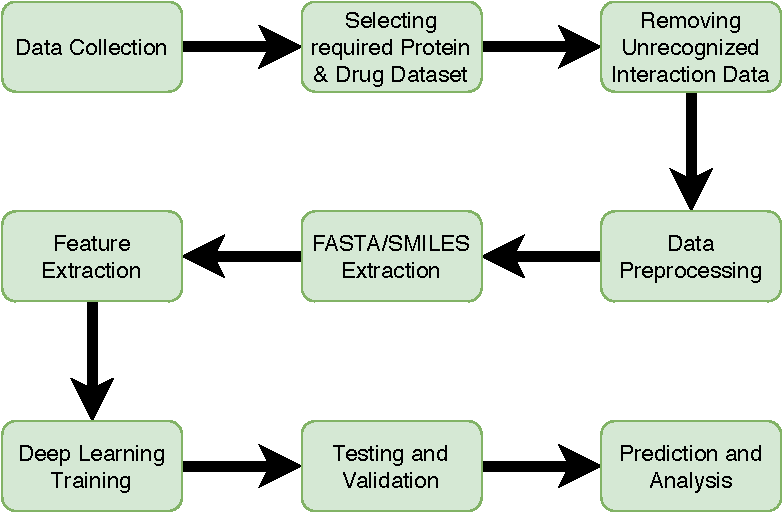
\includegraphics[width=.8\linewidth]{mainmatter/3-Methodology/images/system_block.pdf}
  \caption{System Block Diagram for Protein-Drug Prediction}
  \label{fig:system}
\end{figure}


\subsection{Data Collection}

The dataset is collected from open-internet database. Basically, there are three types of data required in this work: protein, drug and interaction sets. The UniProt Library has been used for extracting proteins features, PubChem for drug features, and NCBI for interaction scores. Additionally, PSI-BLAST is used to generate PSSM matrices for the protein features downloaded.

UniProt contains database of 173,281 proteins of human (Homo sapiens) (until 2019). The protein document consists of the taxonomic classification, identifiers to other databases for cross-linking,  molecular properties, related specific bioactivity, functional property, canonical and isoforms of protein sequence. The protein fasta sequence in particular is of interest to this research. An API can be used to download the available information.  
\url{https://www.uniprot.org/help/programmatic_access}

>O00311

\seqsplit{MEASLGIQMDEPMAFSPQRDRFQAEGSLKKNEQNFKLAGVKKDIEKLYEAVPQLSNVFKIEDKIGEGTFSSVYLATAQLQVGPEEKIALKHLIPTSHPIRIAAELQCLTVAGGQDNVMGVKYCFRKNDHVVIAMPYLEHESFLDILNSLSFQEVREYMLNLFKALKRIHQFGIVHRDVKPSNFLYNRRLKKYALVDFGLAQGTHDTKIELLKFVQSEAQQERCSQNKSHIITGNKIPLSGPVPKELDQQSTTKASVKRPYTNAQIQIKQGKDGKEGSVGLSVQRSVFGERNFNIHSSISHESPAVKLMKQSKTVDVLSRKLATKKKAISTKVMNSAVMRKTASSCPASLTCDCYATDKVCSICLSRRQQVAPRAGTPGFRAPEVLTKCPNQTTAIDMWSAGVIFLSLLSGRYPFYKASDDLTALAQIMTIRGSRETIQAAKTFGKSILCSKEVPAQDLRKLCERLRGMDSSTPKLTSDIQGHASHQPAISEKTDHKASCLVQTPPGQYSGNSFKKGDSNSCEHCFDEYNTNLEGWNEVPDEAYDLLDKLLDLNPASRITAEEALLHPFFKDMSL}

PubCHEM and CHEMBL are drug databases used for feature extraction of drug molecules. PubCHEM is a database containing 96,881,514 drug compounds and associates to each using CID identifier. It allows programmatic access and downloads of database text files. The SMILES structure provided by the PubChem library is used to generate features corresponding to each drug molecule. The properties associated with the molecule is explored using CHEMBL database using a programmatic api request provided. 

\url{https://pubchemdocs.ncbi.nlm.nih.gov/programmatic-access}, 
\url{https://chembl.gitbook.io/chembl-interface-documentation/web-services}. 

\iffalse
UniCHEM is a very useful repository that has been integrated with various web-services. The queries can be done from GET request and JSON text can be retrieved in response to the request. The database can be used to retrieve structure information, mappings, InChIKey and source information related to drug molecule. The InChIKey is used in this work to construct features for small drug molecule (aka ligand).   
\url{https://www.ebi.ac.uk/unichem/rest}
\fi

CHEMBL379218

PubCHEM CID 11314340

\seqsplit{CC1=C2C=C(C=CC2=NN1)C3=CC(=CN=C3)OCC(CC4=CC=CC=C4)N}



For the drug-target interaction (i.e. drug-protein interaction), KIBA scores were used \cite{Tang2013} instead of binary classification. Thus, a regression model was used to predict the drug and protein interaction. The KIBA score regression has two major advantages over binary classification: interaction strength of similarly interacting ligands-target (drugs-protein) can be compared and the bias problem of unknown interactions is refrained \cite{Tang2013,ozturk2018deepdta}. Higher score means that there is more strength of interaction between the two. We use \arabic{no_drugs} ligands as drugs and \arabic{no_proteins} human proteins as target for the prediction problem.

\begin{table}[H]
  \centering
  \caption{KIBA Score Table}
  \begin{tabular}{|l|l|l|l|l|}
    \hline
   
   & O00238 & O00311 & O00329 & O00418  \\ \hline
  CHEMBL10 & 3.518514 & 3.100002 & 4.0 & 3.6  \\ \hline
  CHEMBL102000 & NaN & NaN & NaN & NaN  \\ 
  \hline
  
  \end{tabular}
  \end{table}


Various components were used to form the prediction system. Protein interaction depends on its structural, chemical, molecular(related to H-bond) and electrostatic properties. The structural representation form basis for creating features in other properties. The primary canonical structure of protein-drug set are fed into interaction block. The interaction parameter is filtered accordingly to the filter type. Similarly, the drug feature set are created to be trained with the machine learning algorithm. Finally, after training the training dataset, cross validation of the model was done.

\section{Building Components of Features Processing}

The prediction system is built upon the feature extraction of proteins and drugs. \ref{fig:system2} shows the building components of the Input Vectors for feeding the deep learning network. The KIBA Prediction id done by feeding canonical protein fasta and drug smiles. The other features are constructed on their basis. PSSM matrix is constructed using PSSM matrices of human genome protein library from UniProt~\cite{UniProtConsortium2018} and the protein's FASTA. Two features, \acrfull{et} and \acrfull{pssmdt} are extracted from PSSM. From FASTA, Labelled encodings and \acrfull{rpt} matrix are created. From the SMILES, only labelled encodings is extracted.


\begin{figure}[H]\centering
  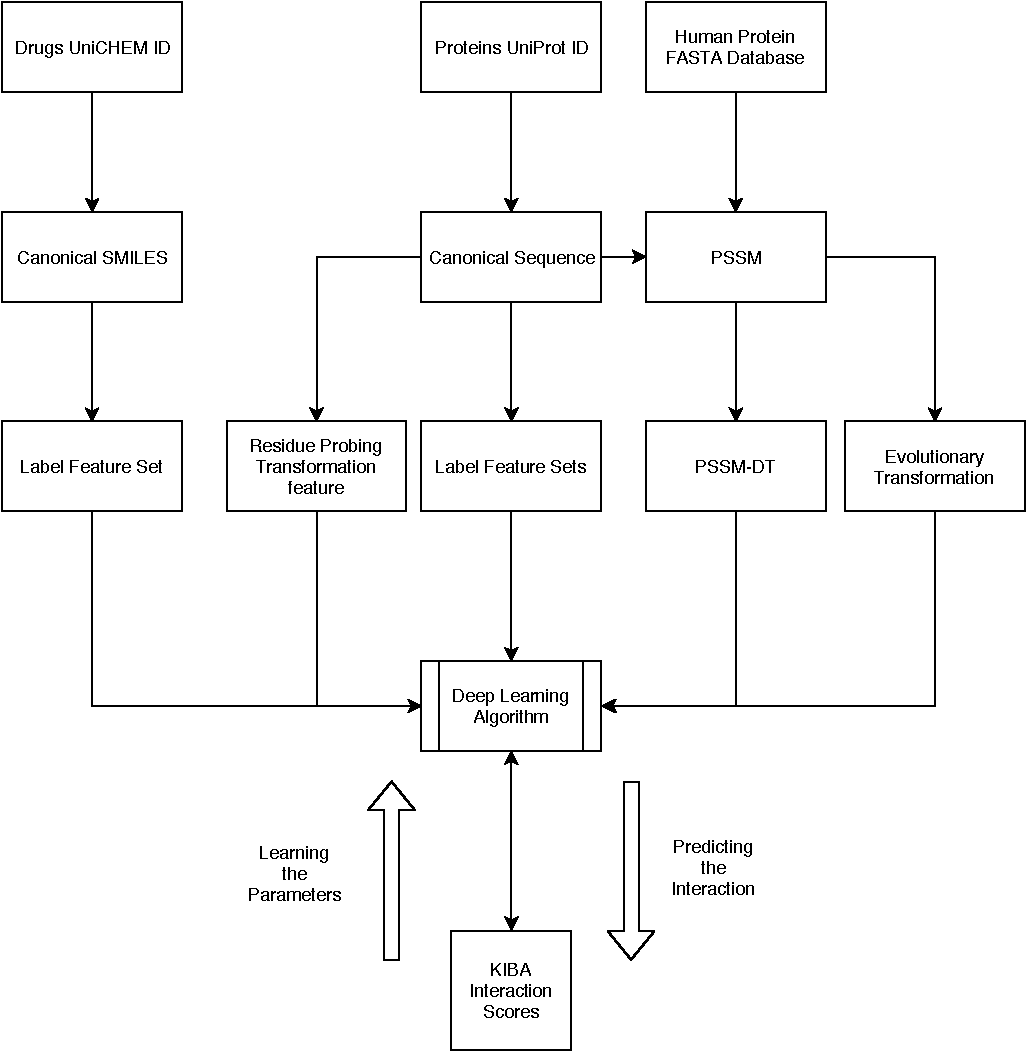
\includegraphics[width=0.9\linewidth]{mainmatter/3-Methodology/images/Algorithm.pdf}
  \caption{Schematic Block Diagram for Protein-Drug Prediction}
  \label{fig:system2}
\end{figure} 




  \section{System Block}

\begin{figure}[h]
  % \def\svgwidth{\columnwidth}
  % \includesvg{mainmatter/3-Methodology/images/block.svg}
  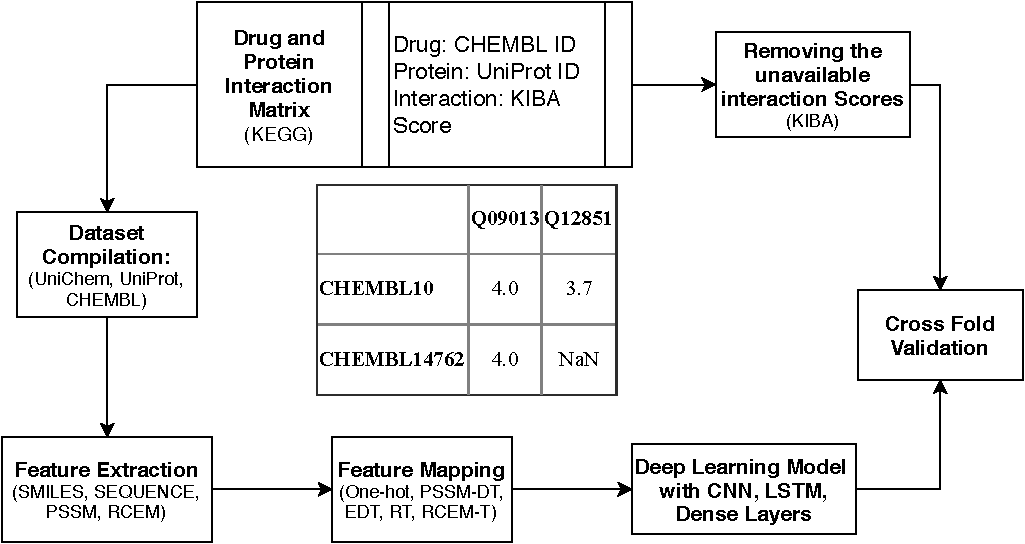
\includegraphics[width=1\linewidth]{mainmatter/3-Methodology/images/block.pdf}
  \caption{Schematic Block Diagram for Protein-Drug Prediction}
  \label{fig:system}
\end{figure}

The Figure ~\ref{fig:system} shows the various components used to form the prediction system. The idea is basic in that protein interaction depends on the structural and chemical properties. The primary canonical structure of protein-drug set are fed into interaction block. The interaction parameter is filtered accordingly to the filter type. Similarly, the drug feature set are created to be trained with the machine learning algorithm. Finally, after training the training dataset, we cross validate the model with test dataset.


\section{Dataset Description}

\iffalse
\subsection{\acrfull{kegg}}
\acrfull{kegg} is a community-driven database which contains large-scale molecular datasets generated by genome sequencing and high-throughput experimental techniuqe.\cite{Kanehisa2000, ozturk2018deepdta} We use \acrshort{kegg} DRUG dataset for finding the interaction set between DRUG and PROTEIN. The interaction score is :
\fi

\subsection{\acrfull{kiba}}
The \acrfull{kiba} Scores are collected from the publicly made available dataset \cite[\textit{Tang. et al.}]{Tang2013}. The scores are actually based on thermodynamic constants K\textsubscript{i} and K\textsubscript{d} and, remaining enzyme activity(Activity \% --  IC\textsubscript{50}) .

% \begin{flushright}
\begin{equation}
  KIBA = \begin{cases}
    K_i . {adj} & \quad {if} \; {IC_{50}\: and\, K_i \,are\, present} \\
    K_b.{adj} & \quad {if}  {IC_{50} \, and \, K_d \, are \, present} \\
    \frac{K_i . {adj} \; K_b.{adj}}{2} & \quad {if\, IC_{50}\,,K_i\, and \,K_d\, are\, present}
  \end{cases}
   \label{eq:kiba}
\end{equation}
where,
\begin{equation}
K_i.{adj} = \frac{IC_{50}}{1 + L_i(IC_{50}/K_i)}
\label{eq:ki_adj}
\end{equation}

\begin{equation}
K_d.{adj} = \frac{IC_{50}}{1 + L_d(IC_{50}/K_d)}
\end{equation}
where L\textsubscript{d} and L\textsubscript{i} are parameters defining weights of IC\textsubscript{50} in model adjustments for K\textsubscript{i} and K\textsubscript{b} 
% \end{flushright}

For a kinase inhibitor drug−target interaction, we consider the medians of three major bioactivity types IC\textsubscript{50}, K\textsubscript{i}, K\textsubscript{d} where
IC\textsubscript{50} \cite{Tang2013} is the concentration at which the inhibitor causes a 50\% inhibition of enzymatic activity and K\textsubscript{i} is defined by \begin{equation}
    Ki = \frac{IC_{50}} {1 + [S]  K_m}
    \label{eq:ki}
\end{equation} 
where,  [{S}] is the experimental substrate concentration and K\textsubscript{m} is the concentration of the substrate.

\iffalse
\begin{equation}
    \tau= \frac{(a−b)}{n(n − 1)/2}   
    \label{eq:tau}
  \end{equation}
  { Here {a} and {b} represent the number of concordant pairs and discordant pairs respectively. }
\fi


All the bioactivity types are available from CHEMBL\cite{Gaulton2017}. Based on interaction data available, we remove the unknown values and get a total of 180244 interaction KIBA score values in the range of -3.09 to 17.8. With the standard deviation of 1.22, it represents a total of \arabic{no_proteins} proteins and \arabic{no_drugs} drugs.

\subsection{Position Specific Score Matrix}

\acrfull{pssm} is a very useful protein feature. The protein feature represented by PSSM depends on the sequence of all the proteins in consideration. The HUMAN genome protein (a database of more than 100,000) is downloaded from UniProt Library. The PSSM matrix is constructed for each of the kinase proteins based on this HUMAN Genome Protein Database. With this, the PSSM matrix is characterized according to human proteins to anticipate the prediction of new identified kinase proteins.

\begin{table}
  \centering
  {\caption{PSSM Analysis Design}
  \label{table:PSSM_Analysis} }
    \subfloat[][Protein FASTA Sequence]{
      \label{table:PSSM_Analysis:fasta} 
      \begin{tabular}{|l|l|} \toprule
      \hline
      1 & GAGGTAAAC \\ \hline
      2 & TCCGTAAGT \\ \hline
      3 & CAGGTTGGA \\ \hline
      4 & ACAGTCAGT \\ \hline
      5 & TAGGTCATT \\ \hline
      6 & TAGGTACTG \\ \hline
      7 & ATGGTAACT \\ \hline
      8 & CAGGTATAC \\ \hline
      9 & TGTGTGAGT \\ \hline
      10 & AAGGTAAGT \\ \hline
      
      \end{tabular}
    }
    \subfloat[][Frequency Table]{
      \label{table:PSSM_Analysis:frequency}
      \begin{tabular}{|l|l|l|l|l|l|l|l|l|l|} \toprule
        \hline
        
         & 1 & 2 & 3 & 4 & 5 & 6 & 7 & 8 & 9 \\ \hline
        A & 3 & 6 & 1 & 0 & 0 & 6 & 7 & 2 & 1 \\ \hline
        C & 2 & 2 & 1 & 0 & 0 & 2 & 1 & 1 & 2 \\ \hline
        G & 1 & 1 & 7 & 10 & 0 & 1 & 1 & 5 & 1 \\ \hline
        T & 4 & 1 & 1 & 0 & 10 & 1 & 1 & 2 & 6 \\ \hline
        
        \end{tabular}

    } 
  
  
  \subfloat[][Log-Likelihood Matrix]{
    % \rule{4cm}{0cm}
    \begin{tabular}{|l|l|l|l|l|l|l|l|l|l|} \toprule
      \hline 
  
          & 1 & 2 & 3 & 4 & 5 & 6 & 7 & 8 & 9 \\ \hline
      A & 0.3 & 0.6 & 0.1 & 0.00 & 0.00 & 0.6 & 0.7 & 0.2 & 0.1 \\ \hline
      C & 0.2 & 0.2 & 0.1 & 0.00 & 0.00 & 0.2 & 0.1 & 0.1 & 0.2 \\ \hline
      G & 0.1 & 0.1 & 0.7 & 1.00 & 0.00 & 0.1 & 0.1 & 0.5 & 0.1 \\ \hline
      T & 0.4 & 0.1 & 0.1 & 0.00 & 1.00 & 0.1 & 0.1 & 0.2 & 0.6 \\ \hline
      
      \end{tabular}  
      \label{table:log_likelihood_pssm}
    }
    
  
  \subfloat[][Sliding Window Score Calculation]{
    \centering
    \begin{tabular}{|l|l|l|l|l|l|l|l|l|l|}
    \hline 
    
        & 1 & 2 & 3 & 4 & 5 & 6 & 7 & 8 & 9 \\ \hline
    A & 0.3 &  &  &  &  &  & 0.7 &  &  \\ \hline
    C &  &  & 0.1 & 0.00 & 0.00 & 0.20 &  &  & 0.2 \\ \hline
    G &  & 0.1 &  &  &  &  &  & 0.5 &  \\ \hline
    T &  &  &  &  &  &  &  &  &  \\ \hline
    
    \end{tabular}  
    \label{table:motif_movement}
    }

    
    \subfloat[][Score of sliding window motifs]{
    \label{wrapTable:pssm-score}
    \begin{tabular}{|l|l|l|l|l|l|l|l|l|l|}
      \hline
      0 & 1 & 2 & 3 & 4 & 5 & 6 & 7 & 8 & 9 \\ \hline
      1.099 & 1 & 2.2 & 2.1 & 2.1 & 1.300 & 1.3 & 1.4 & 2 & 2.9 \\ \hline
      \end{tabular}
    }
\end{table}

Table \ref{table:PSSM_Analysis} shows a conventional process of calculating PSSM score values. The sequence following shows the process of calculating the scores once the PSSM distribution of the whole family is calculated. Table \ref{table:motif_movement} shows the score distribution of lowercase amino acid sequence (starting after 4th position) determined by the size of the sliding window.

\seqsplit{ACTC\textbf{agccccagc}GGAGGTGAAGGACGTCCTTCCCCAGGAGCCGGTGAGAAGCGCAGTCGGGGGCACGGGGATGAGCTCAGGGGCCTCTAGAAAGATGTAGCTGGGACCTCGGGAAGCCCTGGCCTCCAGGTAGTCTCAGGAGAGCTACTCAGGGTCGGGCTTGGGGAGAGGAGGAGCGGGGGTGAGGCCAGCAGCA} 

% % \begin{wraptable}{br}{5.5cm}
% \begin{table}[H]
%     \centering
    
% \end{table}
% % \end{wraptable}

.3, .1, .1, 0, 0, .2, .7, .5, .2  == Sum(2.1) - posix(4) -- See table \ref{wrapTable:pssm-score}

\begin{figure}[htbp]
    \centering 
          %  \subfloat[]{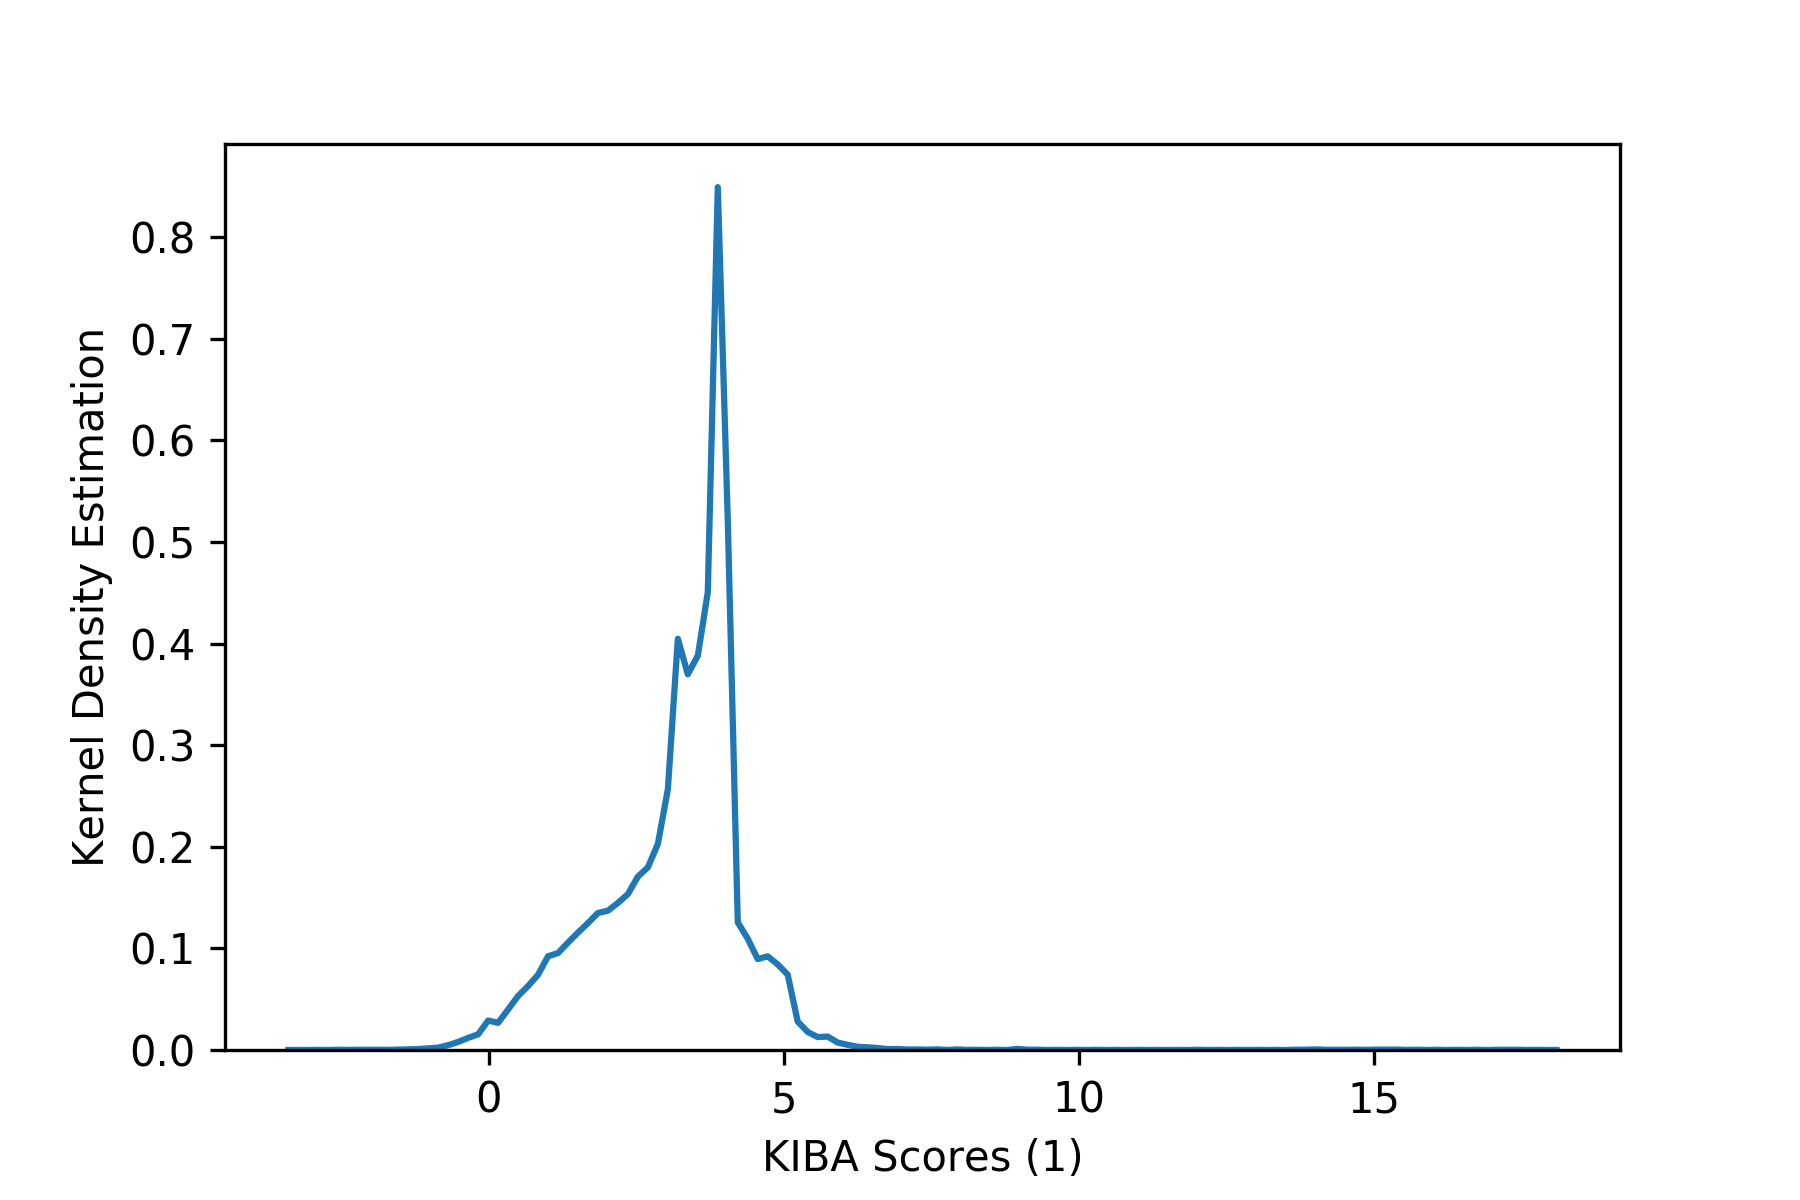
\includegraphics[width=.3\textwidth]{dataset/images/KIBA_scores.png}}
          
           \subfloat[][Drug-Protein Interaction]{
             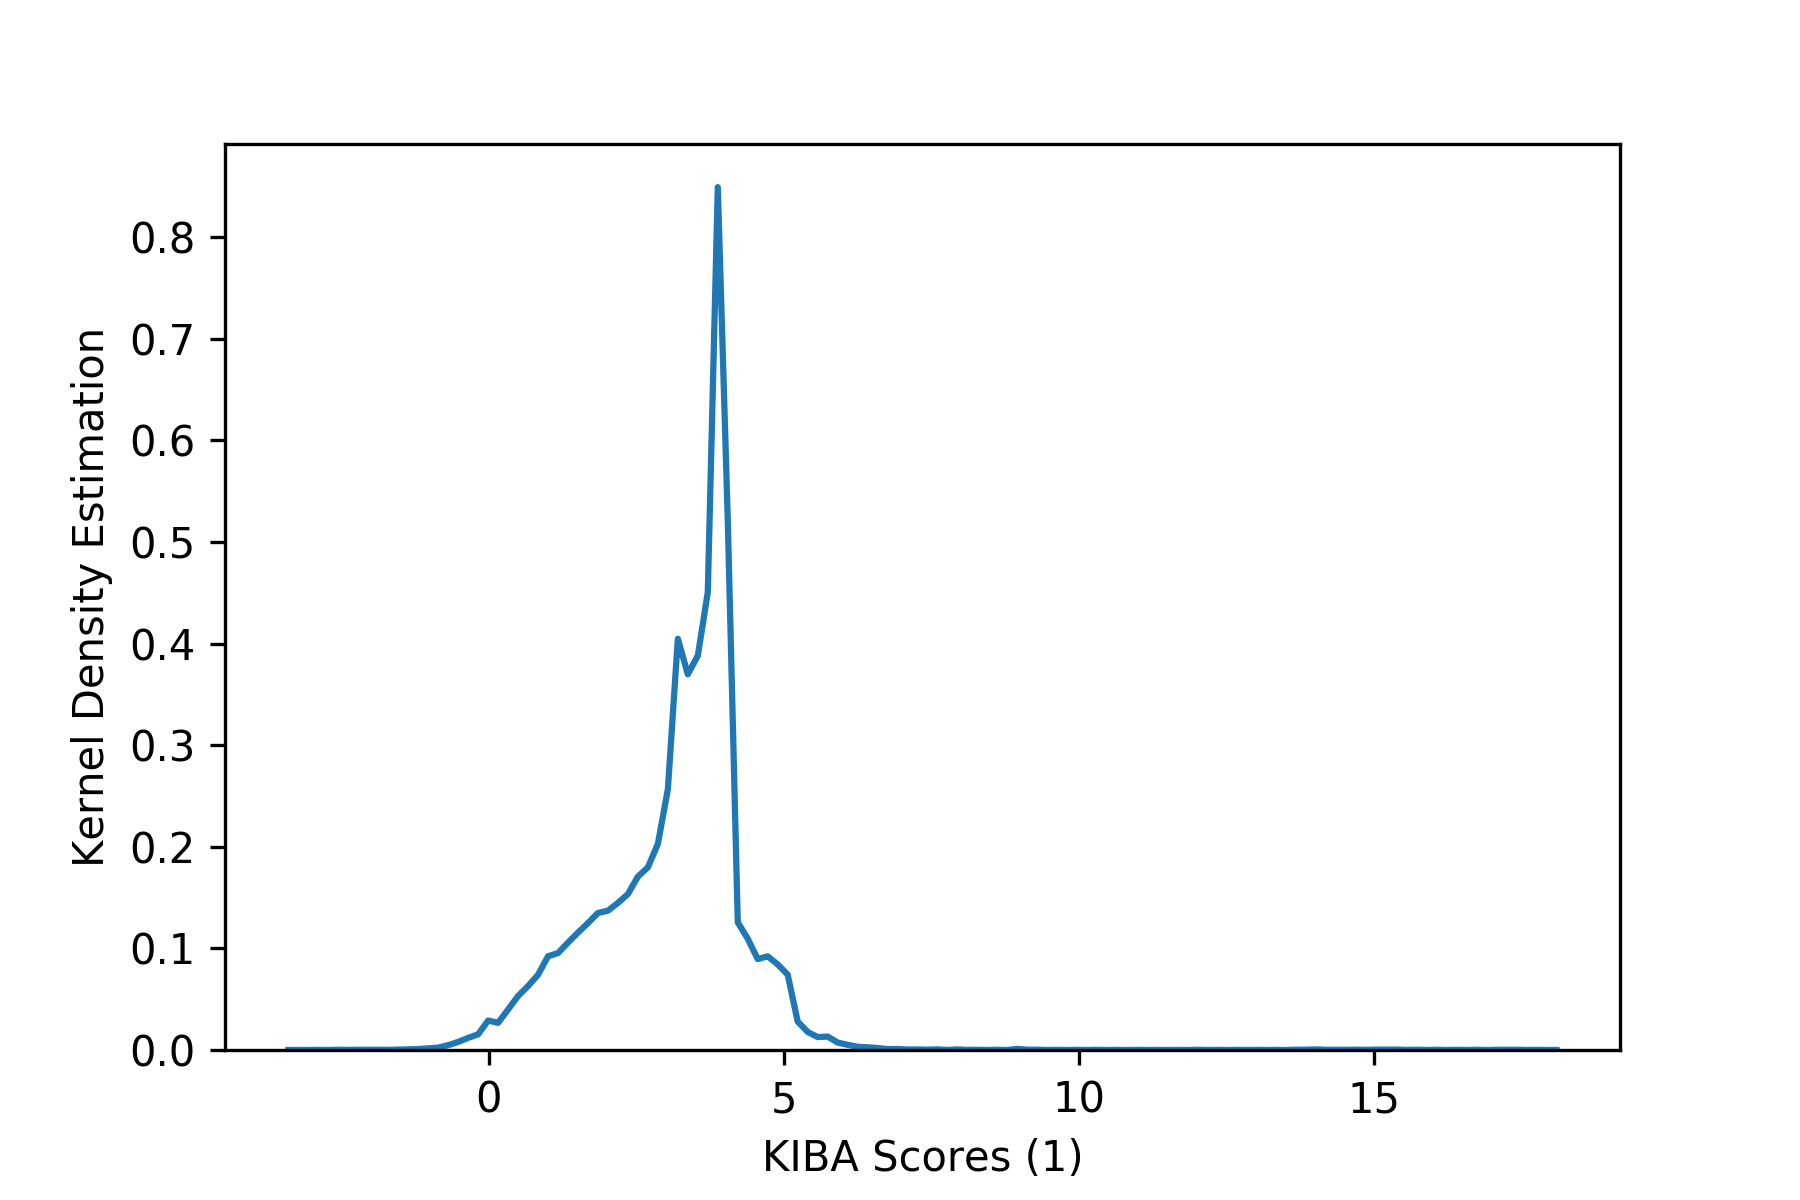
\includegraphics[width=.5\textwidth]{dataset/images/KIBA_scores.png}
             \label{fig:kiba_scores}
             }

           \subfloat[][Drugs SMILES Sequence]{
            \label{fig:drug_dist}  
            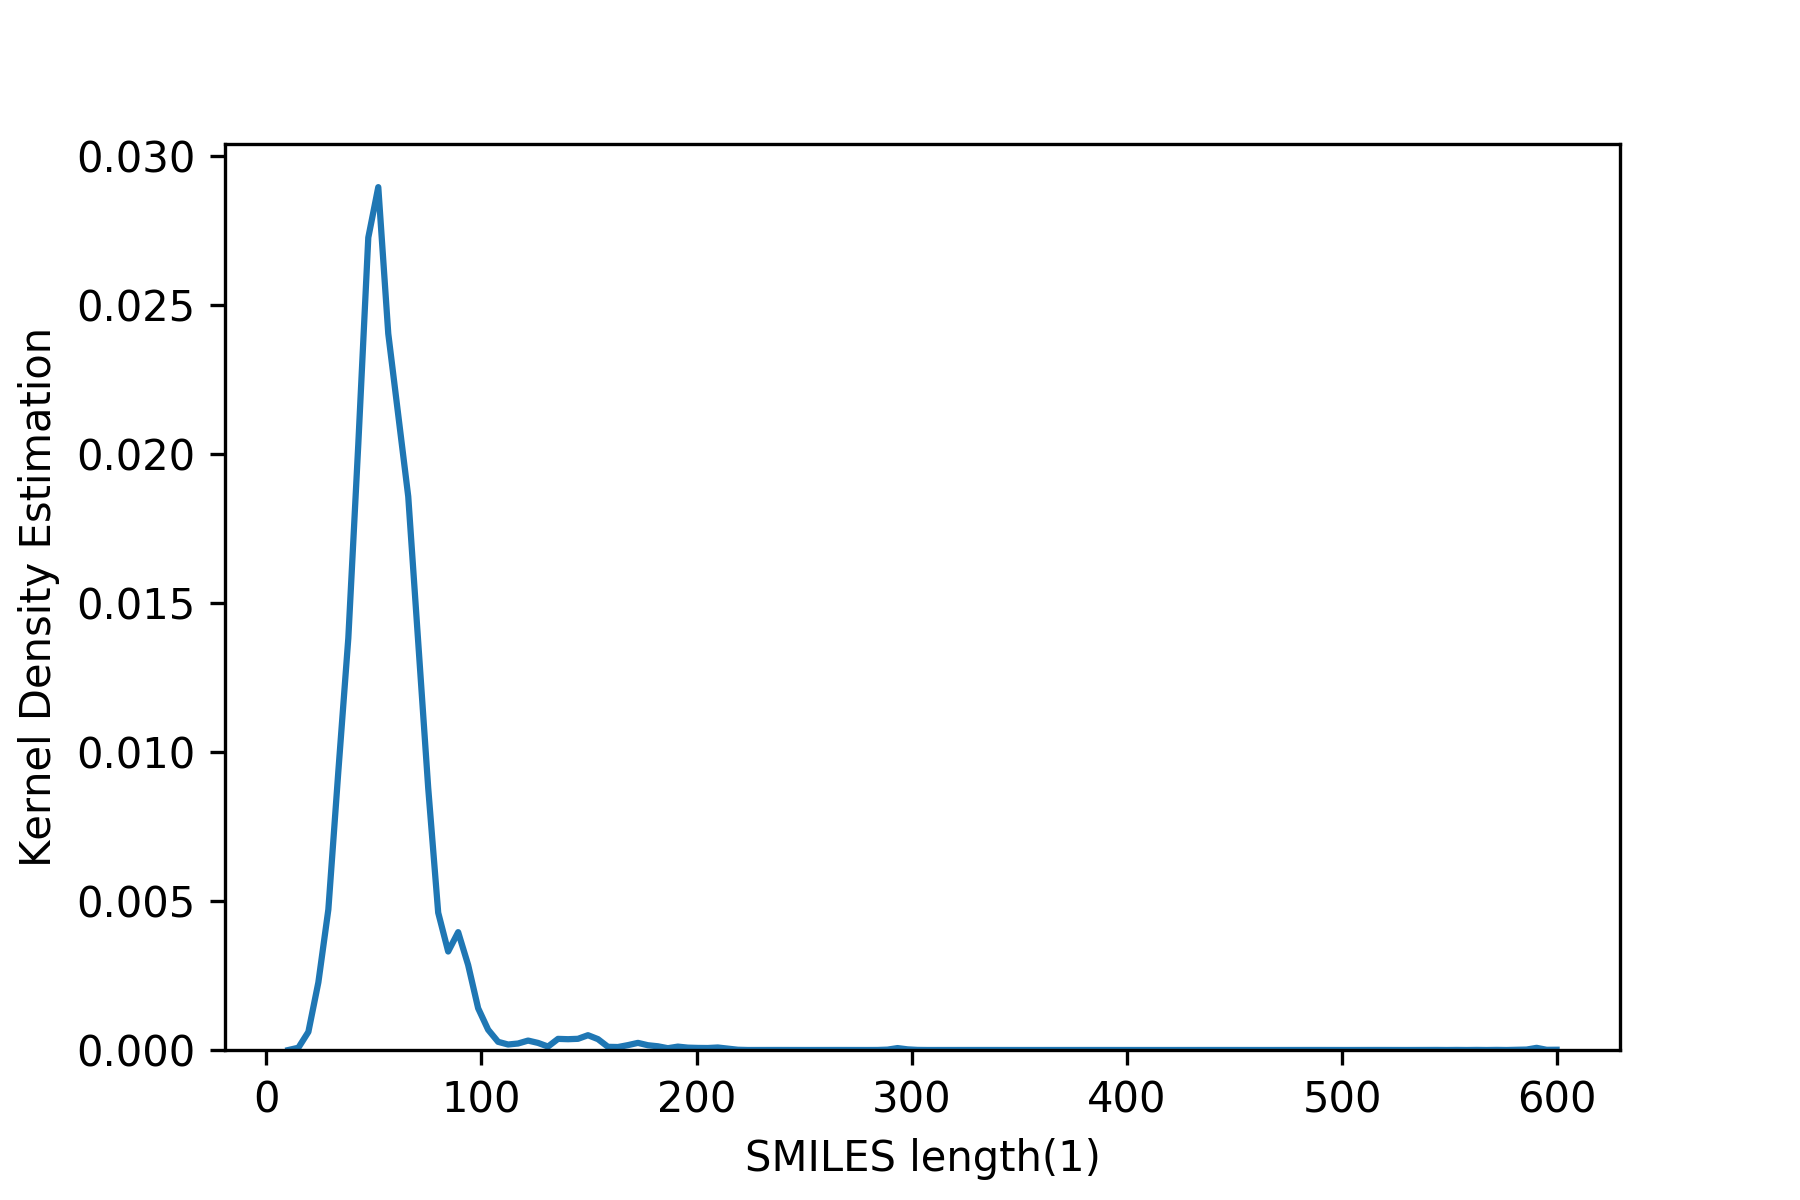
\includegraphics[width=.5\textwidth]{dataset/images/SMILES_distribution.png}
            }

           \subfloat[][Protein FASTA Sequence]{
             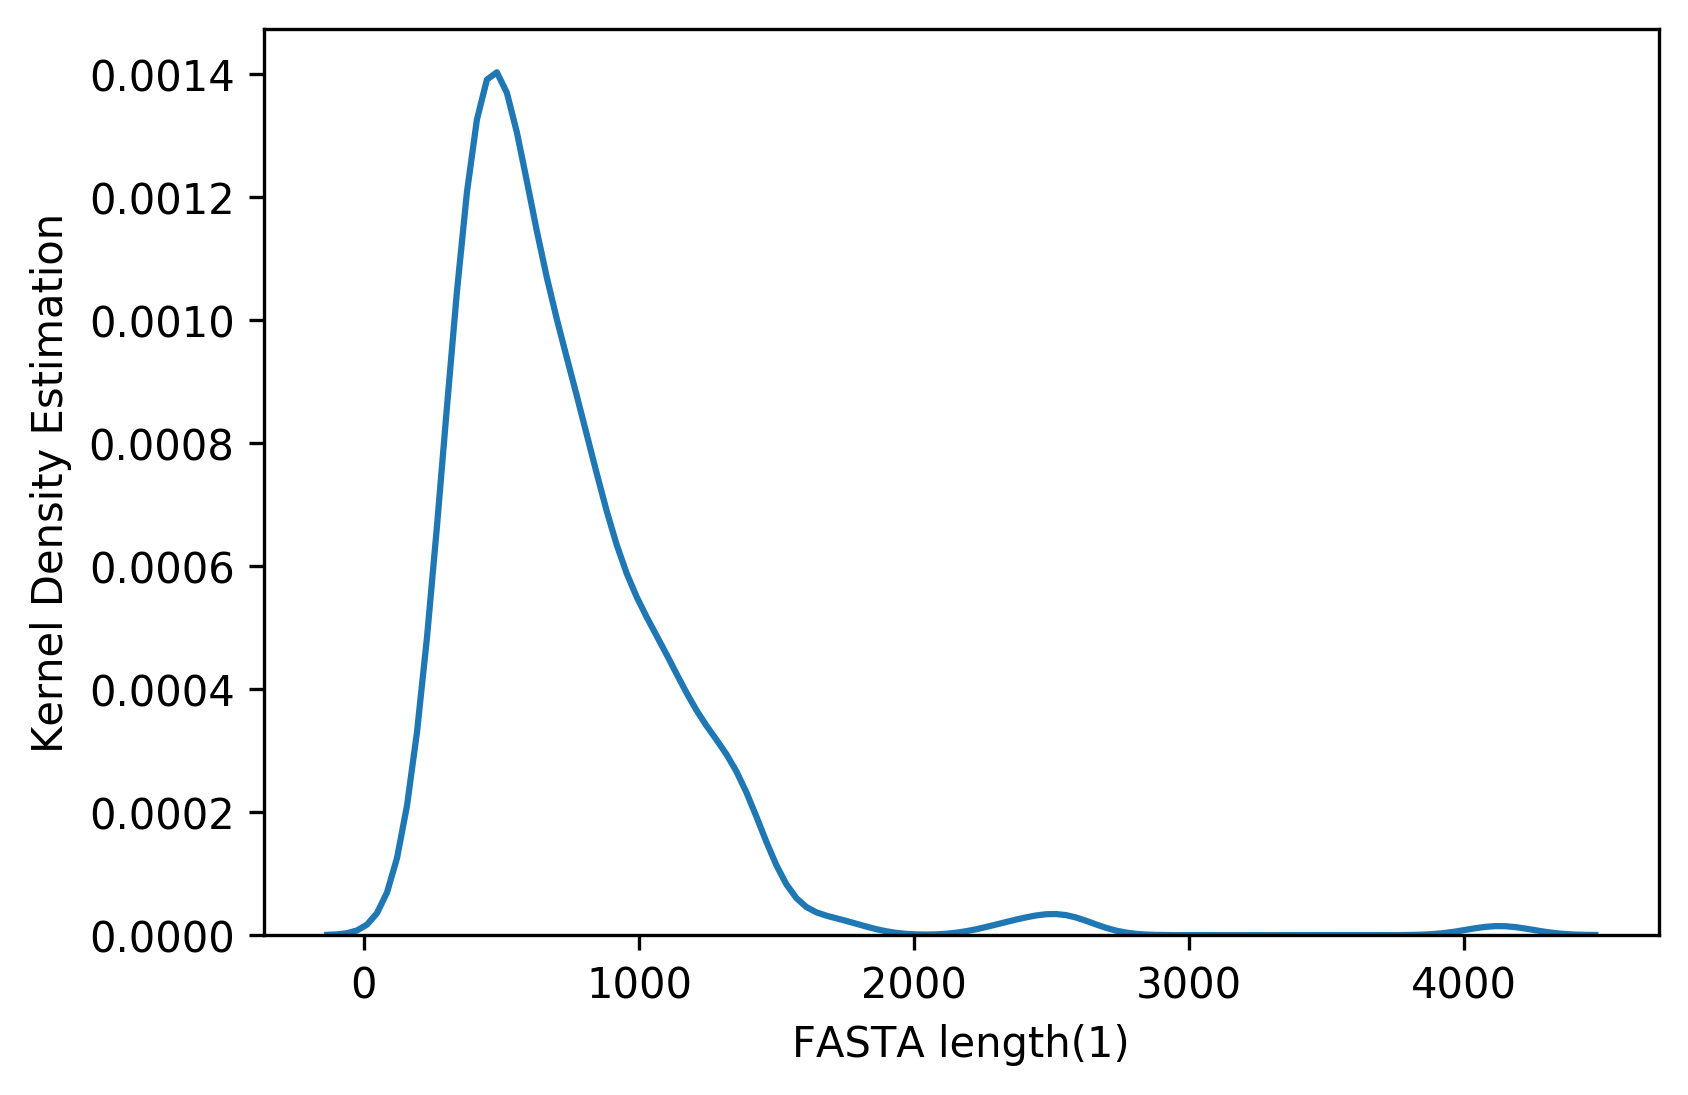
\includegraphics[width=.5\textwidth]{dataset/images/FASTA_distribution.png}
             \label{fig:prot_dist}
            }

           \caption[KDE Distribution]{Kernel Density Estimation Distribution of KIBA-interaction scores of Drug Sequences and Protein Sequences. \ref{sub@fig:kiba_scores} Distribution of KIBA Scores in Protein-Drug Interaction Pair, \ref{sub@fig:drug_dist} Distribution of length in Labeled Encodings of Drug Sequence, \ref{sub@fig:prot_dist} Distribution of length in Labelled Encodings Protein Sequence }
           \label{fig:kiba_drug_protein}
\end{figure}
  
\iffalse
  \subsection{UniProt and CHEMBL}
  
  \subsubsection{UniProt} 
  The sequence related information of protein is referenced using UniProt Identifier and protein sequence (FASTA) is called using the api from UniProt. \cite{UniProtConsortium2018}
  
  
  \subsubsection{CHEMBL}
  The molecular fingerprints related to drugs are referenced usning CHEMBL Identifier and the drug sequence is called from CHEMBL database. \cite{Gaulton2017}
  \fi
  \subsection{PSI-BLAST}
  PSI-Blast tools relates with multiple sequence alignments from a family of protein sequences\cite{Schaffer2001}. This helps to create a \acrshort{pssm} - Equation (\ref{eq:pssm}) - matrix referred to as secondary protein structure. For this study, the PSSM profile of every protein sequence is obtained by executing iteration of PSI-BLAST against \cite[KEGG]{Schaffer2001} protein. PSSM profile is a matrix of L*20 dimensions whereby 20 is the standard type of amino acids and L being the length of the protein. The larger positive scores represent conserved positions, which in turn implies critical functional residues that are required to perform various intermolecular interactions.\cite[PSSM]{Schaffer2001}
  
  \begin{equation}
    PSSM = \begin{bmatrix}
      P_{1,1} & P_{1,2} & \dots & P_{1,20} \\
      P_{2,1} & P_{2,2} & \dots & P_{2,20} \\
      \vdots  & \vdots  & \ddots & \vdots \\
      P_{L,1} & P_{L,2} & \dots & P_{L,20} \\
    \end{bmatrix}
    \label{eq:pssm}
  \end{equation}
  
  \subsubsection{PSSM-DT}
  Two forms of \acrshort{pssm} distance transformation techniques are used to transform the \acrshort{pssm} information into fixed dimensional vectors \cite{Xu2015}. The PSSM-DT (PSSM-Distance Transformation) can transform the \acrshort{pssm} information into uniform numeric representation by approximately measuring the occurrence probabilities of any pairs of amino acid. It results in two types of feature matrices: PSSM-SDT and PSSM-DDT defined by:
  
  \begin{equation}[H]
    PSSM-SDT(i,lg) = \sum_{i=1}^{L-lg} S_{i,j} \times \frac{ S_{i,j+lg} }{L-lg} 
    \label{eq:pssmsdt}
  \end{equation}
  \textit{\center lg =  distance of separation between same amino acid sequence}
  
  \begin{equation}[H]
    PSSM-DDT(i_1,i_2, lg) = \sum_{j=1}^{L-lg} S_{i_1,j} \times \frac{ S_{i_2,j+lg} }{ L-lg} 
    \label{eq:pssmddt}
  \end{equation}
  \textit{\centering i\textsubscript{1} and i\textsubscript{2} refer to tow different types of amino acids}
  
  Thus we have [380 ~\eqref{eq:pssmddt}+20 ~\eqref{eq:pssmsdt} = 400] x lg matrix which will be used as protein-specific vector in this work.
  
  \subsubsection{Evolutionary Distance Transformation Matrix}
  The mutational information of protein can be more informative than the sequence information itself\cite{Zhang2014}. Evolutionary difference formula (EDF) is used to represent mutation difference between adjacent residues. Secondly, the PSSM is converted into 20 x 20 matrix (ED-PSSM). These extracts are the non co-occurrence probability for two amino acids separated by a certain distance \textit{d} in the protein from the PSSM profile. For example, d=1 implies that the two amino acids are consecutive; d=2 implies that there is one amino acid between the two. Next, the EDT feature vector computed from ED-PSSM can be represented as (~\ref{eq:Pmat}): 
  \begin{equation}
    \label{eq:Pmat}
    P = [ \partial_1 ,\partial_2, \dots, \partial_\Omega]
  \end{equation}
  where $\Omega$ is an integer that represents the dimension of the vector whose value is 400.. The non-co-occurrence probability of two amino acids separated by distance \textit{d} can be computed as:
  \begin{equation}
    f(A_x,A_y) = \sum_{d=1}^{D} \frac{1}{L-d} \sum_{i=1}^{L-d} (P_{i,x} - P_{i+d,y})^2
    \label{eq:edt}
  \end{equation}
  where $P_{i,x}$ and $P_{i+d,y}$ are the elements in the PSSM profile; $A_x$ and $A_y$ represent any of the the 20 different amino acids in the protein sequence. Finally we spread the $f(A_x,A_y)$ in equation ~\ref{eq:Pmat} as:
  $ \partial_1 = f(A_1,A_2) $, 
  $ \partial_{400} = f(A_{20}, A_{20}) $
  
  
  \subsection{Residue feature} 
  The Statistical Residue Vector Space \acrshort{srv} \cite{Wong2018} plays an important role in Residue Residue Interaction and creates a basis for structural stability of the protein sequence itself. It is related to the tertiary structure of the protein sequence. Nonetheless, another function is to create a correlated sequence of information whereby two proteins are distantly related by sequence. Simultaneously, it is highly related to the functional characteristic of protein.  With this, table ~\ref{table:r2r} as attached in Appendix depicts a 20 x 20 matrix whose rows and columns represent 20 standard amino acids.
  
  \subsubsection{Residue Probing Transformation(RPT) feature}
  RPT as proposed by Jeong et al.\cite{Jeong2011}, and implemented by Pujan et al.\cite{Mishra2019}, emphasize domains with similar conservation rates by grouping domain families based on their conservation score in the PSSM profile.
  \begin{equation}
    RPT = \begin{bmatrix}
      S_{1,1} & S_{1,2} & \dots & S_{1,20} \\
      S_{2,1} & S_{2,2} & \dots & S_{2,20} \\
      \vdots  & \vdots  & \ddots & \vdots \\
      S_{2,1} & S_{2,2} & \dots & S_{2,20} \\
    \end{bmatrix}
    \label{eq:rpt}
  \end{equation}
  The RPT matrix (Equation ~\ref{eq:rpt}) is then tranformed into feature vector of 400 dimensions, as shown in Equation ~\ref{eq:rptV}.
  
  \begin{equation}
    V = [ f_{s_{1,1}}, f_{s_{1,2}}, \dots, f_{s_{i,j}}, \dots, f_{s_{20,20}} ]
    \label{eq:rptV}
  \end{equation}
  where, 
  \begin{equation}
    f_{s_{i,j}} = \frac{s_{i,j}}{L} (i,j = 1,2,\dots,20)
    \label{eq:rptF}
  \end{equation}

  \subsection{Labelled Encodings}
  
  The labeled encoding techniques is used to represent the canonical structure of drugs and proteins. The structural canonical information is preserved while sending the feature set to deep learning method. An array of integers are formed from particular sequence while representing the structural information.
  
  The Labelled Encodings of protein and drugs can be defined by table \ref{table:label_encoding} :
  \begin{table}[H]
    \centering
    \caption{Labeled Encoding of Proteins and Drugs}
    \label{table:label_encoding}
    \qquad
    \subfloat[][Label Encodings for Proteins]{
      \label{table:label_encoding:prot}
      \begin{tabular}{|cccc|}
        \hline
        A --> 1 & C --> 2 & B --> 3 & E --> 4 \\ \hline
        D --> 5 & G --> 6 & F --> 7 & I --> 8 \\ \hline
      \end{tabular}
      }

    \qquad
    \subfloat[][Label Encodings for Drugs]{
      \label{table:label_encoding:drugs}
      \centering
      % \caption{Drugs Labeled Encoding Technique}
      \begin{tabular}{|cccc|}
        \hline
        \# --> 1 & \% --> 2 & : --> 3 & + --> 5 \\ \hline
        4 --> 13 & 7 --> 14 & F --> 25 & I --> 26 \\ \hline
      \end{tabular}
      }
  \end{table}
  
  % CHARPROTSET = { "A": 1, "C": 2, "B": 3, "E": 4, "D": 5, "G": 6,
	% 			"F": 7, "I": 8, "H": 9, "K": 10, "M": 11, "L": 12,
	% 			"O": 13, "N": 14, "Q": 15, "P": 16, "S": 17, "R": 18,
	% 			"U": 19, "T": 20, "W": 21,
	% 			"V": 22, "Y": 23, "X": 24,
	% 			"Z": 25 }

  % CHARCANSMISET = { "#": 1, "%": 2, ")": 3, "(": 4, "+": 5, "-": 6,
	% 		 ".": 7, "1": 8, "0": 9, "3": 10, "2": 11, "5": 12,
	% 		 "4": 13, "7": 14, "6": 15, "9": 16, "8": 17, "=": 18,
	% 		 "A": 19, "C": 20, "B": 21, "E": 22, "D": 23, "G": 24,
	% 		 "F": 25, "I": 26, "H": 27, "K": 28, "M": 29, "L": 30,
	% 		 "O": 31, "N": 32, "P": 33, "S": 34, "R": 35, "U": 36,
	% 		 "T": 37, "W": 38, "V": 39, "Y": 40, "[": 41, "Z": 42,
	% 		 "]": 43, "_": 44, "a": 45, "c": 46, "b": 47, "e": 48,
	% 		 "d": 49, "g": 50, "f": 51, "i": 52, "h": 53, "m": 54,
	% 		 "l": 55, "o": 56, "n": 57, "s": 58, "r": 59, "u": 60,
	% 		 "t": 61, "y": 62 }
  
  \subsection{Position Specific Score Matrix}

\acrfull{pssm} is a very useful protein feature. The protein feature represented by PSSM depends on the sequence of all the proteins in consideration. The HUMAN genome protein (a database of more than 100,000) is downloaded from UniProt Library. The PSSM matrix is constructed for each of the kinase proteins based on this HUMAN Genome Protein Database. With this, the PSSM matrix is characterized according to human proteins to anticipate the prediction of new identified kinase proteins.

\begin{table}
  \centering
  {\caption{PSSM Analysis Design}
  \label{table:PSSM_Analysis} }
    \subfloat[][Protein FASTA Sequence]{
      \label{table:PSSM_Analysis:fasta} 
      \begin{tabular}{|l|l|} \toprule
      \hline
      1 & GAGGTAAAC \\ \hline
      2 & TCCGTAAGT \\ \hline
      3 & CAGGTTGGA \\ \hline
      4 & ACAGTCAGT \\ \hline
      5 & TAGGTCATT \\ \hline
      6 & TAGGTACTG \\ \hline
      7 & ATGGTAACT \\ \hline
      8 & CAGGTATAC \\ \hline
      9 & TGTGTGAGT \\ \hline
      10 & AAGGTAAGT \\ \hline
      
      \end{tabular}
    }
    \subfloat[][Frequency Table]{
      \label{table:PSSM_Analysis:frequency}
      \begin{tabular}{|l|l|l|l|l|l|l|l|l|l|} \toprule
        \hline
        
         & 1 & 2 & 3 & 4 & 5 & 6 & 7 & 8 & 9 \\ \hline
        A & 3 & 6 & 1 & 0 & 0 & 6 & 7 & 2 & 1 \\ \hline
        C & 2 & 2 & 1 & 0 & 0 & 2 & 1 & 1 & 2 \\ \hline
        G & 1 & 1 & 7 & 10 & 0 & 1 & 1 & 5 & 1 \\ \hline
        T & 4 & 1 & 1 & 0 & 10 & 1 & 1 & 2 & 6 \\ \hline
        
        \end{tabular}

    } 
  
  
  \subfloat[][Log-Likelihood Matrix]{
    % \rule{4cm}{0cm}
    \begin{tabular}{|l|l|l|l|l|l|l|l|l|l|} \toprule
      \hline 
  
          & 1 & 2 & 3 & 4 & 5 & 6 & 7 & 8 & 9 \\ \hline
      A & 0.3 & 0.6 & 0.1 & 0.00 & 0.00 & 0.6 & 0.7 & 0.2 & 0.1 \\ \hline
      C & 0.2 & 0.2 & 0.1 & 0.00 & 0.00 & 0.2 & 0.1 & 0.1 & 0.2 \\ \hline
      G & 0.1 & 0.1 & 0.7 & 1.00 & 0.00 & 0.1 & 0.1 & 0.5 & 0.1 \\ \hline
      T & 0.4 & 0.1 & 0.1 & 0.00 & 1.00 & 0.1 & 0.1 & 0.2 & 0.6 \\ \hline
      
      \end{tabular}  
      \label{table:log_likelihood_pssm}
    }
    
  
  \subfloat[][Sliding Window Score Calculation]{
    \centering
    \begin{tabular}{|l|l|l|l|l|l|l|l|l|l|}
    \hline 
    
        & 1 & 2 & 3 & 4 & 5 & 6 & 7 & 8 & 9 \\ \hline
    A & 0.3 &  &  &  &  &  & 0.7 &  &  \\ \hline
    C &  &  & 0.1 & 0.00 & 0.00 & 0.20 &  &  & 0.2 \\ \hline
    G &  & 0.1 &  &  &  &  &  & 0.5 &  \\ \hline
    T &  &  &  &  &  &  &  &  &  \\ \hline
    
    \end{tabular}  
    \label{table:motif_movement}
    }

    
    \subfloat[][Score of sliding window motifs]{
    \label{wrapTable:pssm-score}
    \begin{tabular}{|l|l|l|l|l|l|l|l|l|l|}
      \hline
      0 & 1 & 2 & 3 & 4 & 5 & 6 & 7 & 8 & 9 \\ \hline
      1.099 & 1 & 2.2 & 2.1 & 2.1 & 1.300 & 1.3 & 1.4 & 2 & 2.9 \\ \hline
      \end{tabular}
    }
\end{table}

Table \ref{table:PSSM_Analysis} shows a conventional process of calculating PSSM score values. The sequence following shows the process of calculating the scores once the PSSM distribution of the whole family is calculated. Table \ref{table:motif_movement} shows the score distribution of lowercase amino acid sequence (starting after 4th position) determined by the size of the sliding window.

\seqsplit{ACTC\textbf{agccccagc}GGAGGTGAAGGACGTCCTTCCCCAGGAGCCGGTGAGAAGCGCAGTCGGGGGCACGGGGATGAGCTCAGGGGCCTCTAGAAAGATGTAGCTGGGACCTCGGGAAGCCCTGGCCTCCAGGTAGTCTCAGGAGAGCTACTCAGGGTCGGGCTTGGGGAGAGGAGGAGCGGGGGTGAGGCCAGCAGCA} 

% % \begin{wraptable}{br}{5.5cm}
% \begin{table}[H]
%     \centering
    
% \end{table}
% % \end{wraptable}

.3, .1, .1, 0, 0, .2, .7, .5, .2  == Sum(2.1) - posix(4) -- See table \ref{wrapTable:pssm-score}

\begin{figure}[htbp]
    \centering 
          %  \subfloat[]{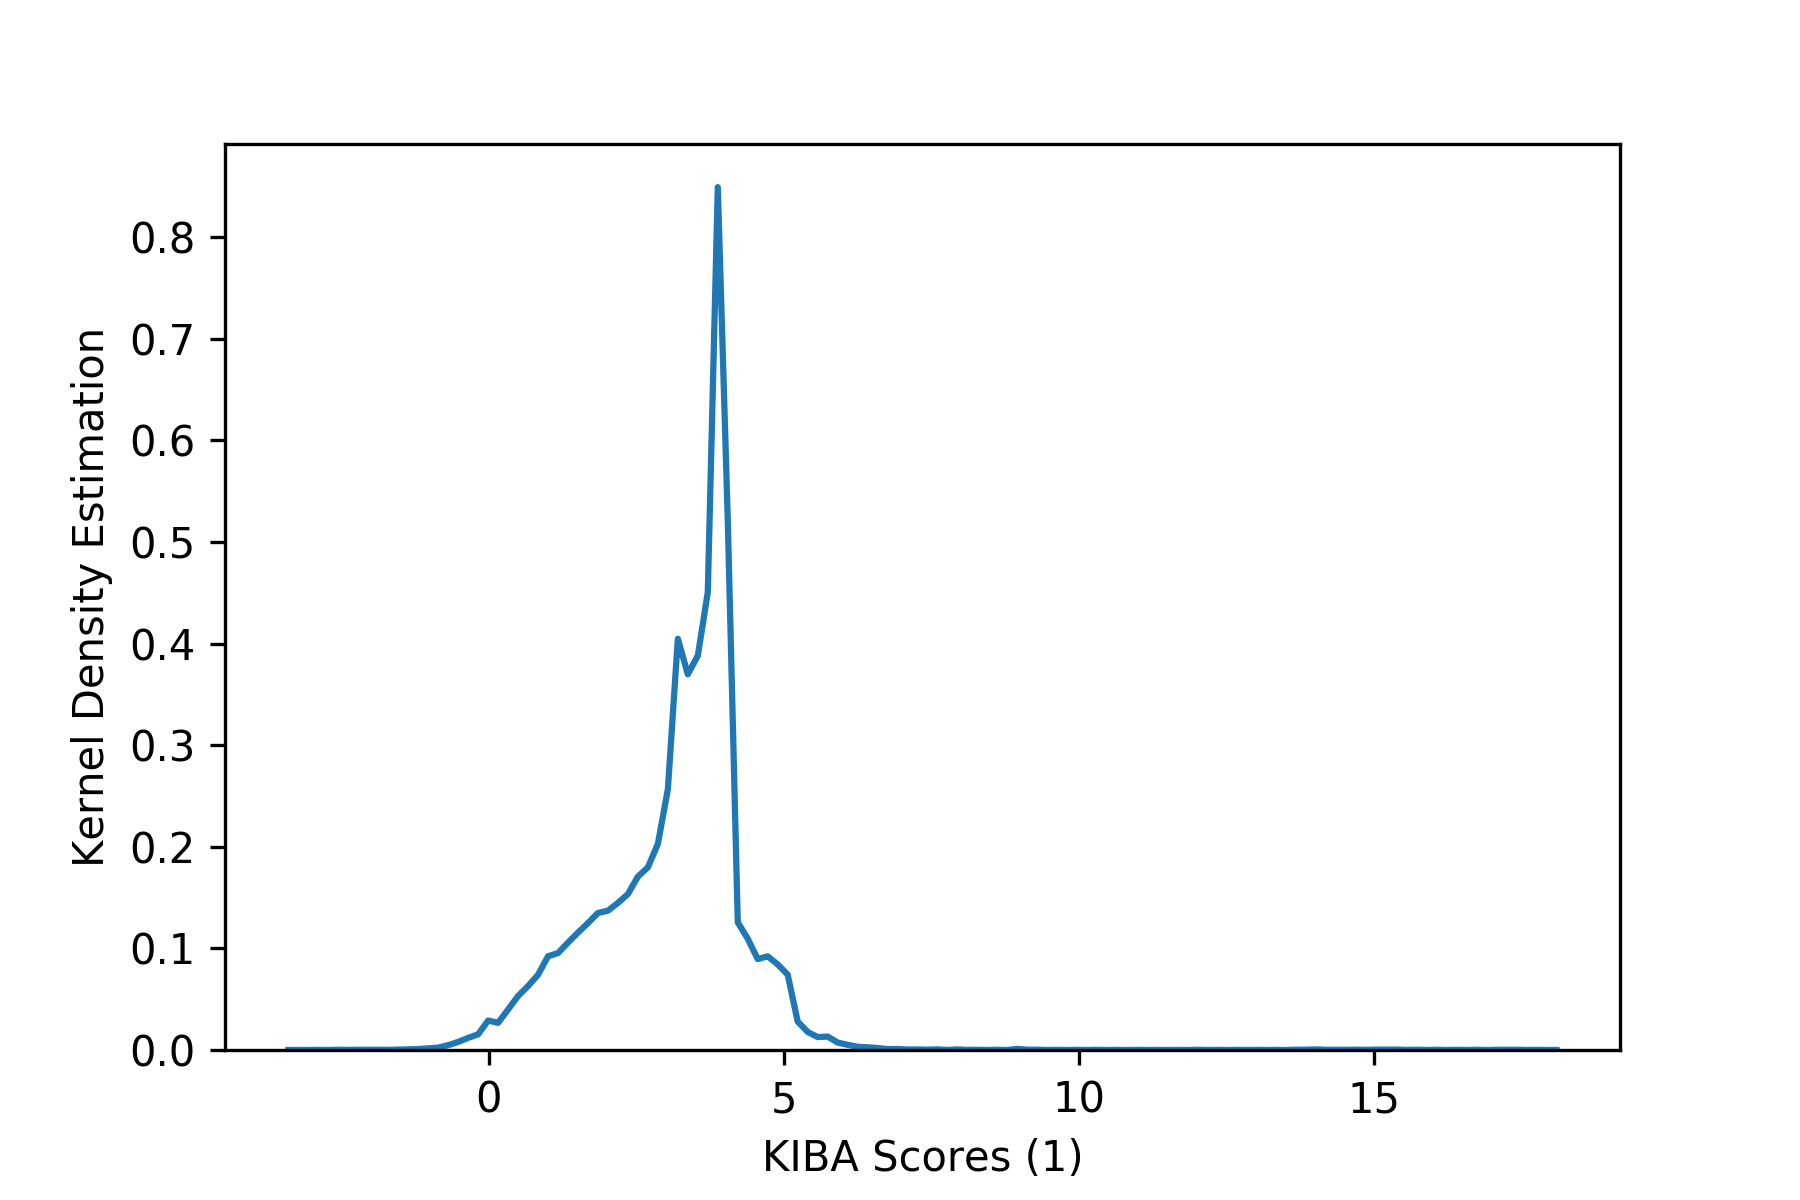
\includegraphics[width=.3\textwidth]{dataset/images/KIBA_scores.png}}
          
           \subfloat[][Drug-Protein Interaction]{
             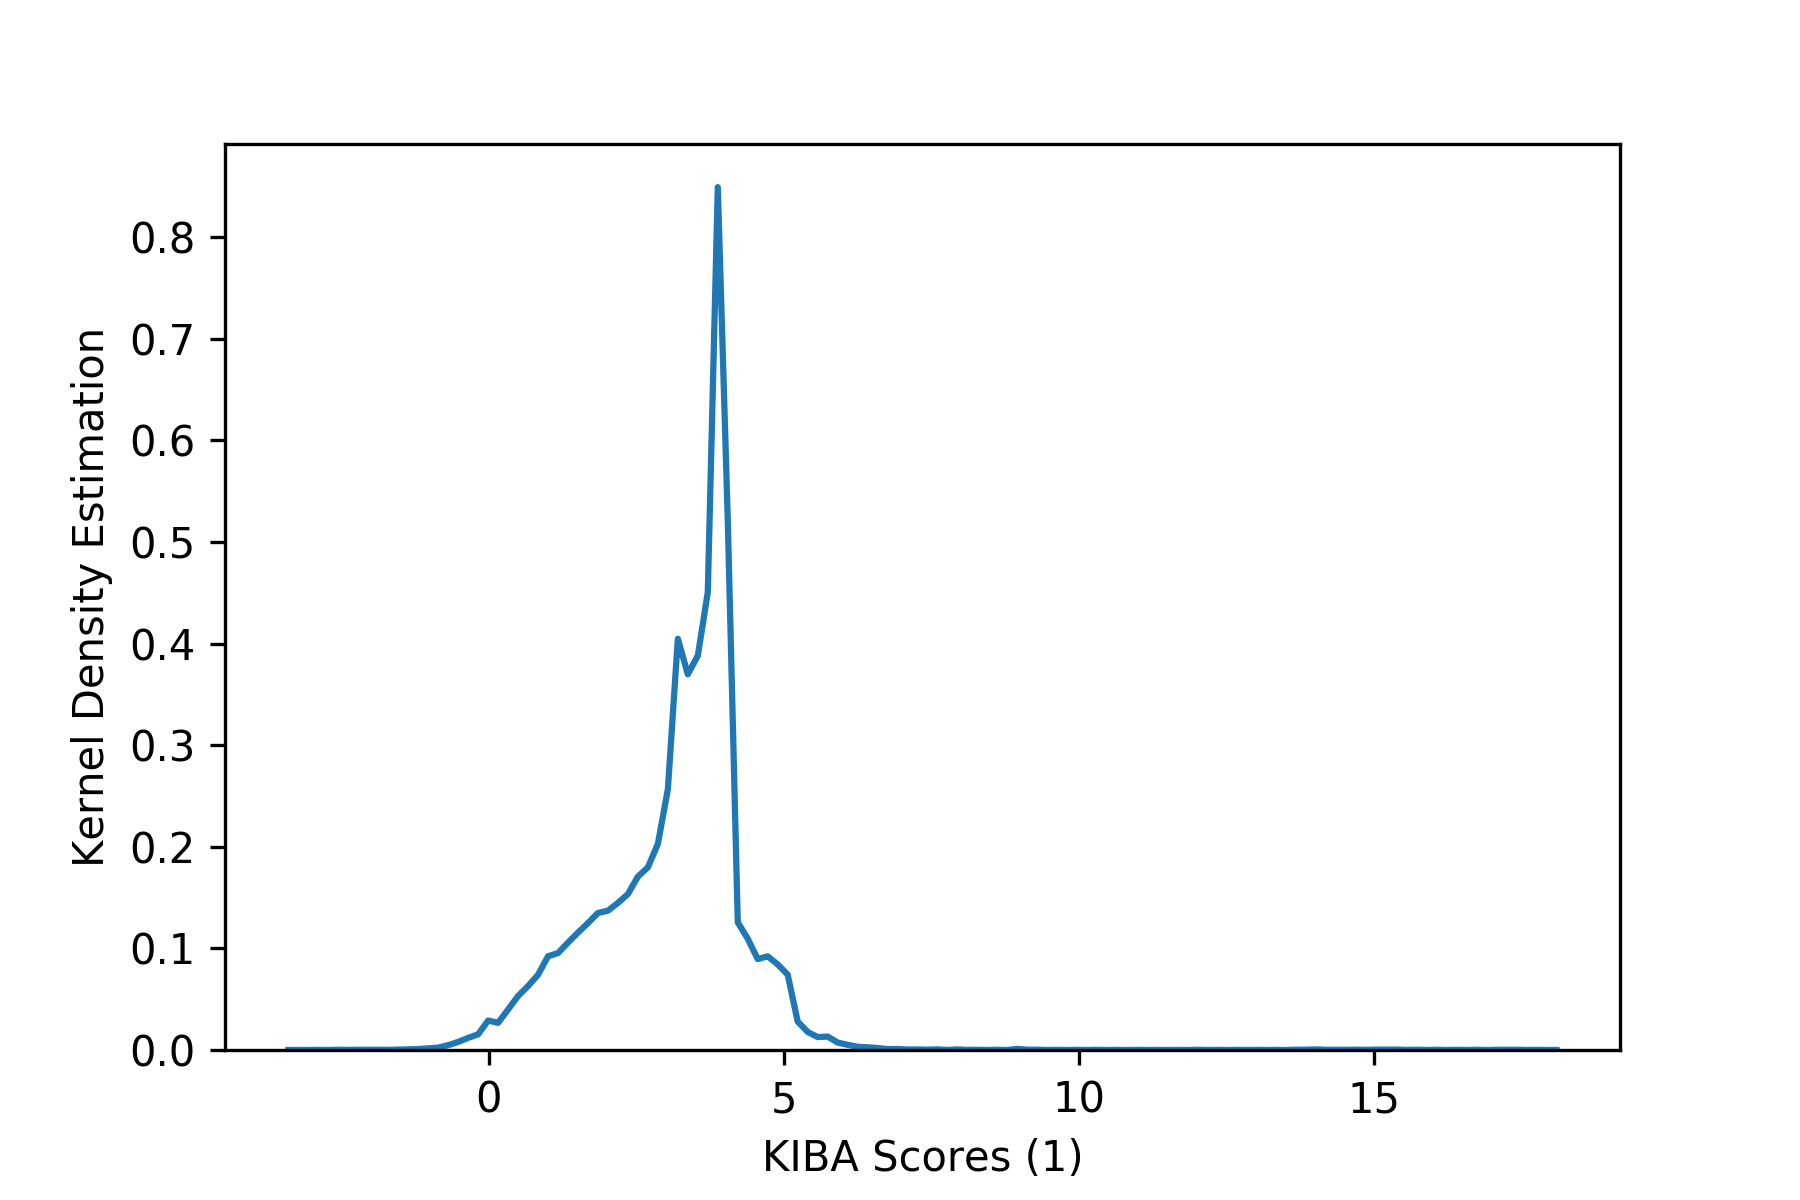
\includegraphics[width=.5\textwidth]{dataset/images/KIBA_scores.png}
             \label{fig:kiba_scores}
             }

           \subfloat[][Drugs SMILES Sequence]{
            \label{fig:drug_dist}  
            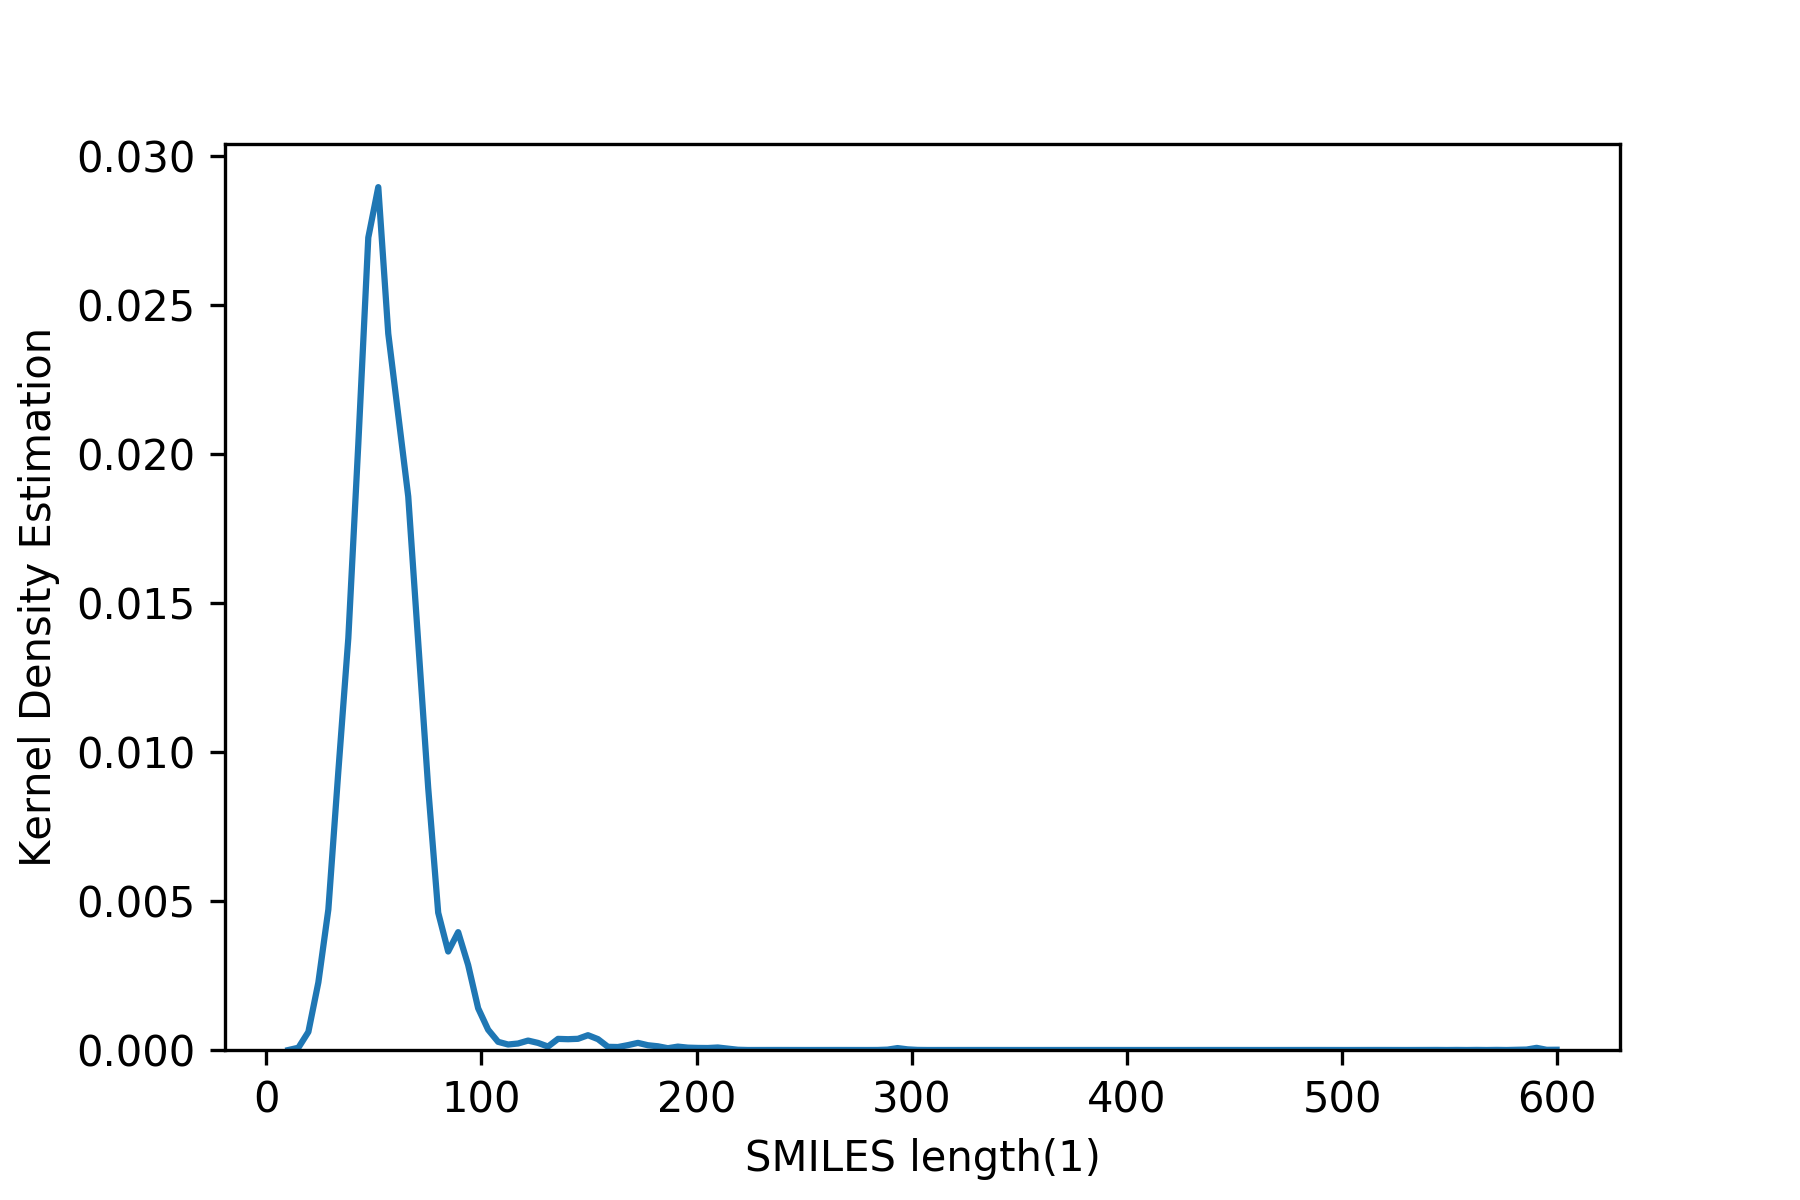
\includegraphics[width=.5\textwidth]{dataset/images/SMILES_distribution.png}
            }

           \subfloat[][Protein FASTA Sequence]{
             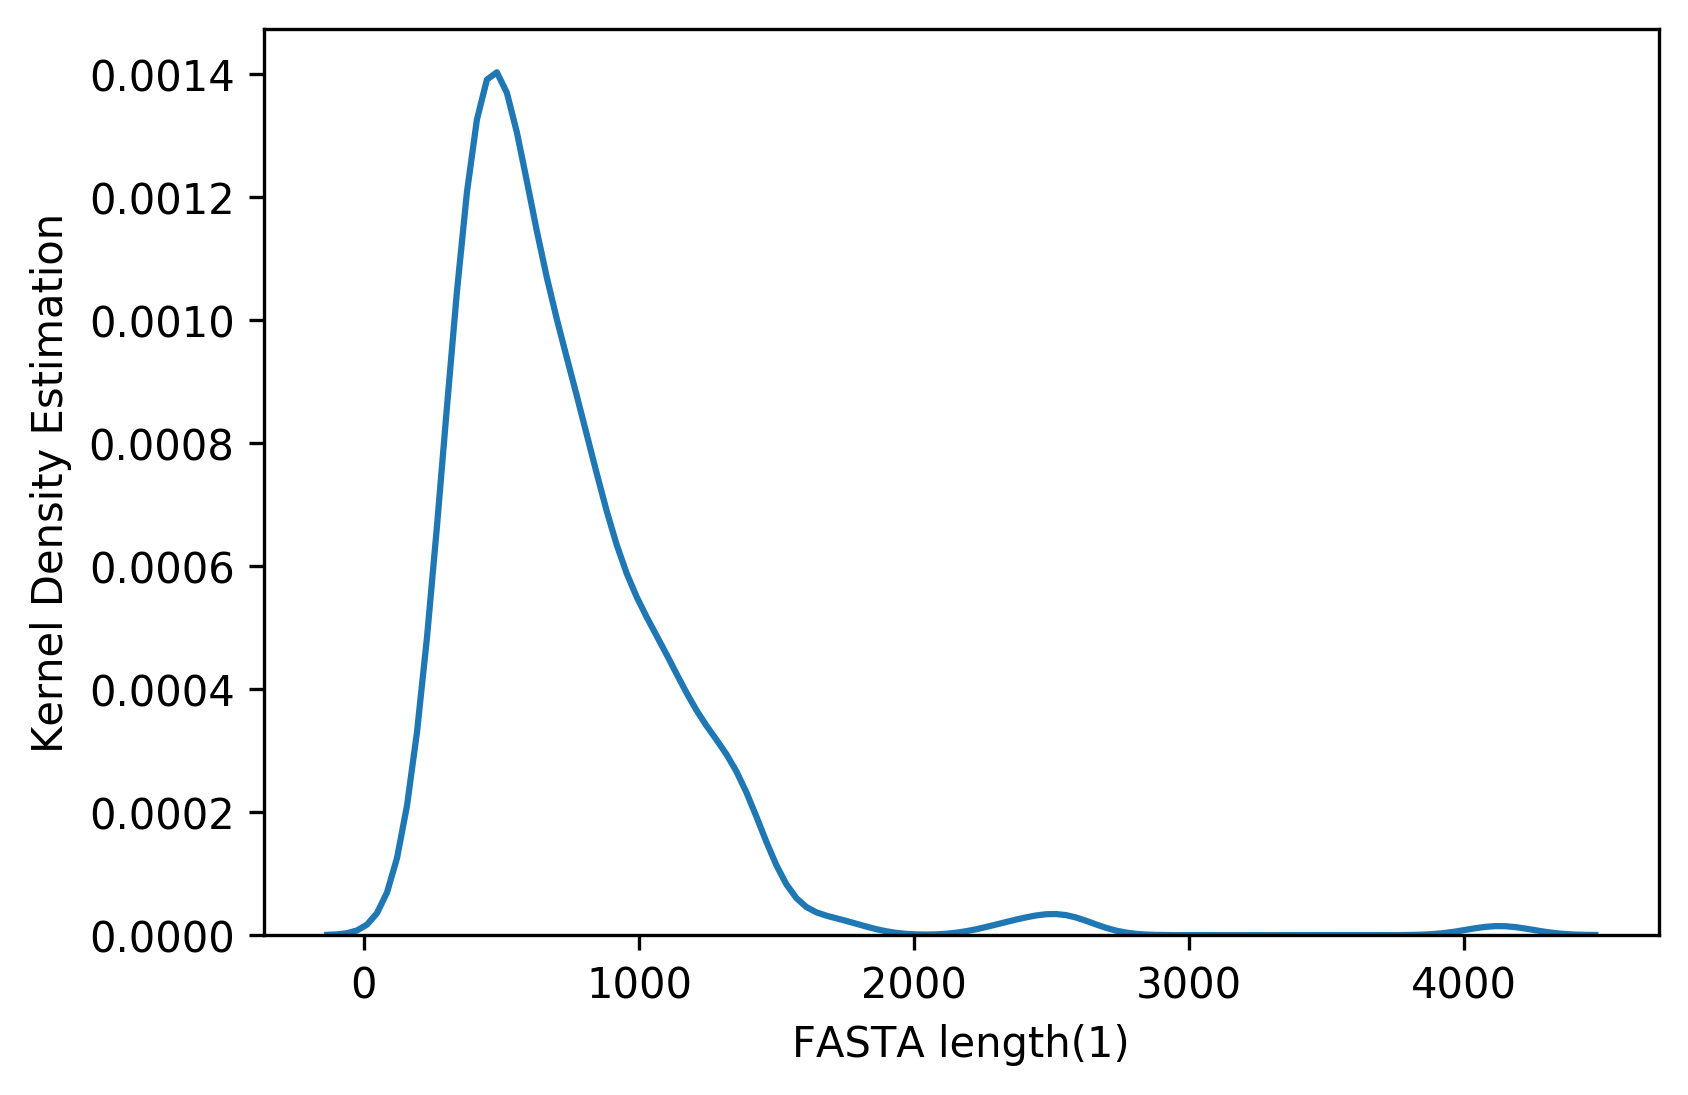
\includegraphics[width=.5\textwidth]{dataset/images/FASTA_distribution.png}
             \label{fig:prot_dist}
            }

           \caption[KDE Distribution]{Kernel Density Estimation Distribution of KIBA-interaction scores of Drug Sequences and Protein Sequences. \ref{sub@fig:kiba_scores} Distribution of KIBA Scores in Protein-Drug Interaction Pair, \ref{sub@fig:drug_dist} Distribution of length in Labeled Encodings of Drug Sequence, \ref{sub@fig:prot_dist} Distribution of length in Labelled Encodings Protein Sequence }
           \label{fig:kiba_drug_protein}
\end{figure}
  
\iffalse
  \subsection{UniProt and CHEMBL}
  
  \subsubsection{UniProt} 
  The sequence related information of protein is referenced using UniProt Identifier and protein sequence (FASTA) is called using the api from UniProt. \cite{UniProtConsortium2018}
  
  
  \subsubsection{CHEMBL}
  The molecular fingerprints related to drugs are referenced usning CHEMBL Identifier and the drug sequence is called from CHEMBL database. \cite{Gaulton2017}
  \fi
  \subsection{PSI-BLAST}
  PSI-Blast tools relates with multiple sequence alignments from a family of protein sequences\cite{Schaffer2001}. This helps to create a \acrshort{pssm} - Equation (\ref{eq:pssm}) - matrix referred to as secondary protein structure. For this study, the PSSM profile of every protein sequence is obtained by executing iteration of PSI-BLAST against \cite[KEGG]{Schaffer2001} protein. PSSM profile is a matrix of L*20 dimensions whereby 20 is the standard type of amino acids and L being the length of the protein. The larger positive scores represent conserved positions, which in turn implies critical functional residues that are required to perform various intermolecular interactions.\cite[PSSM]{Schaffer2001}
  
  \begin{equation}
    PSSM = \begin{bmatrix}
      P_{1,1} & P_{1,2} & \dots & P_{1,20} \\
      P_{2,1} & P_{2,2} & \dots & P_{2,20} \\
      \vdots  & \vdots  & \ddots & \vdots \\
      P_{L,1} & P_{L,2} & \dots & P_{L,20} \\
    \end{bmatrix}
    \label{eq:pssm}
  \end{equation}
  
  \subsubsection{PSSM-DT}
  Two forms of \acrshort{pssm} distance transformation techniques are used to transform the \acrshort{pssm} information into fixed dimensional vectors \cite{Xu2015}. The PSSM-DT (PSSM-Distance Transformation) can transform the \acrshort{pssm} information into uniform numeric representation by approximately measuring the occurrence probabilities of any pairs of amino acid. It results in two types of feature matrices: PSSM-SDT and PSSM-DDT defined by:
  
  \begin{equation}[H]
    PSSM-SDT(i,lg) = \sum_{i=1}^{L-lg} S_{i,j} \times \frac{ S_{i,j+lg} }{L-lg} 
    \label{eq:pssmsdt}
  \end{equation}
  \textit{\center lg =  distance of separation between same amino acid sequence}
  
  \begin{equation}[H]
    PSSM-DDT(i_1,i_2, lg) = \sum_{j=1}^{L-lg} S_{i_1,j} \times \frac{ S_{i_2,j+lg} }{ L-lg} 
    \label{eq:pssmddt}
  \end{equation}
  \textit{\centering i\textsubscript{1} and i\textsubscript{2} refer to tow different types of amino acids}
  
  Thus we have [380 ~\eqref{eq:pssmddt}+20 ~\eqref{eq:pssmsdt} = 400] x lg matrix which will be used as protein-specific vector in this work.
  
  \subsubsection{Evolutionary Distance Transformation Matrix}
  The mutational information of protein can be more informative than the sequence information itself\cite{Zhang2014}. Evolutionary difference formula (EDF) is used to represent mutation difference between adjacent residues. Secondly, the PSSM is converted into 20 x 20 matrix (ED-PSSM). These extracts are the non co-occurrence probability for two amino acids separated by a certain distance \textit{d} in the protein from the PSSM profile. For example, d=1 implies that the two amino acids are consecutive; d=2 implies that there is one amino acid between the two. Next, the EDT feature vector computed from ED-PSSM can be represented as (~\ref{eq:Pmat}): 
  \begin{equation}
    \label{eq:Pmat}
    P = [ \partial_1 ,\partial_2, \dots, \partial_\Omega]
  \end{equation}
  where $\Omega$ is an integer that represents the dimension of the vector whose value is 400.. The non-co-occurrence probability of two amino acids separated by distance \textit{d} can be computed as:
  \begin{equation}
    f(A_x,A_y) = \sum_{d=1}^{D} \frac{1}{L-d} \sum_{i=1}^{L-d} (P_{i,x} - P_{i+d,y})^2
    \label{eq:edt}
  \end{equation}
  where $P_{i,x}$ and $P_{i+d,y}$ are the elements in the PSSM profile; $A_x$ and $A_y$ represent any of the the 20 different amino acids in the protein sequence. Finally we spread the $f(A_x,A_y)$ in equation ~\ref{eq:Pmat} as:
  $ \partial_1 = f(A_1,A_2) $, 
  $ \partial_{400} = f(A_{20}, A_{20}) $
  
  
  \subsection{Residue feature} 
  The Statistical Residue Vector Space \acrshort{srv} \cite{Wong2018} plays an important role in Residue Residue Interaction and creates a basis for structural stability of the protein sequence itself. It is related to the tertiary structure of the protein sequence. Nonetheless, another function is to create a correlated sequence of information whereby two proteins are distantly related by sequence. Simultaneously, it is highly related to the functional characteristic of protein.  With this, table ~\ref{table:r2r} as attached in Appendix depicts a 20 x 20 matrix whose rows and columns represent 20 standard amino acids.
  
  \subsubsection{Residue Probing Transformation(RPT) feature}
  RPT as proposed by Jeong et al.\cite{Jeong2011}, and implemented by Pujan et al.\cite{Mishra2019}, emphasize domains with similar conservation rates by grouping domain families based on their conservation score in the PSSM profile.
  \begin{equation}
    RPT = \begin{bmatrix}
      S_{1,1} & S_{1,2} & \dots & S_{1,20} \\
      S_{2,1} & S_{2,2} & \dots & S_{2,20} \\
      \vdots  & \vdots  & \ddots & \vdots \\
      S_{2,1} & S_{2,2} & \dots & S_{2,20} \\
    \end{bmatrix}
    \label{eq:rpt}
  \end{equation}
  The RPT matrix (Equation ~\ref{eq:rpt}) is then tranformed into feature vector of 400 dimensions, as shown in Equation ~\ref{eq:rptV}.
  
  \begin{equation}
    V = [ f_{s_{1,1}}, f_{s_{1,2}}, \dots, f_{s_{i,j}}, \dots, f_{s_{20,20}} ]
    \label{eq:rptV}
  \end{equation}
  where, 
  \begin{equation}
    f_{s_{i,j}} = \frac{s_{i,j}}{L} (i,j = 1,2,\dots,20)
    \label{eq:rptF}
  \end{equation}

  \subsection{Labelled Encodings}
  
  The labeled encoding techniques is used to represent the canonical structure of drugs and proteins. The structural canonical information is preserved while sending the feature set to deep learning method. An array of integers are formed from particular sequence while representing the structural information.
  
  The Labelled Encodings of protein and drugs can be defined by table \ref{table:label_encoding} :
  \begin{table}[H]
    \centering
    \caption{Labeled Encoding of Proteins and Drugs}
    \label{table:label_encoding}
    \qquad
    \subfloat[][Label Encodings for Proteins]{
      \label{table:label_encoding:prot}
      \begin{tabular}{|cccc|}
        \hline
        A --> 1 & C --> 2 & B --> 3 & E --> 4 \\ \hline
        D --> 5 & G --> 6 & F --> 7 & I --> 8 \\ \hline
      \end{tabular}
      }

    \qquad
    \subfloat[][Label Encodings for Drugs]{
      \label{table:label_encoding:drugs}
      \centering
      % \caption{Drugs Labeled Encoding Technique}
      \begin{tabular}{|cccc|}
        \hline
        \# --> 1 & \% --> 2 & : --> 3 & + --> 5 \\ \hline
        4 --> 13 & 7 --> 14 & F --> 25 & I --> 26 \\ \hline
      \end{tabular}
      }
  \end{table}
  
  % CHARPROTSET = { "A": 1, "C": 2, "B": 3, "E": 4, "D": 5, "G": 6,
	% 			"F": 7, "I": 8, "H": 9, "K": 10, "M": 11, "L": 12,
	% 			"O": 13, "N": 14, "Q": 15, "P": 16, "S": 17, "R": 18,
	% 			"U": 19, "T": 20, "W": 21,
	% 			"V": 22, "Y": 23, "X": 24,
	% 			"Z": 25 }

  % CHARCANSMISET = { "#": 1, "%": 2, ")": 3, "(": 4, "+": 5, "-": 6,
	% 		 ".": 7, "1": 8, "0": 9, "3": 10, "2": 11, "5": 12,
	% 		 "4": 13, "7": 14, "6": 15, "9": 16, "8": 17, "=": 18,
	% 		 "A": 19, "C": 20, "B": 21, "E": 22, "D": 23, "G": 24,
	% 		 "F": 25, "I": 26, "H": 27, "K": 28, "M": 29, "L": 30,
	% 		 "O": 31, "N": 32, "P": 33, "S": 34, "R": 35, "U": 36,
	% 		 "T": 37, "W": 38, "V": 39, "Y": 40, "[": 41, "Z": 42,
	% 		 "]": 43, "_": 44, "a": 45, "c": 46, "b": 47, "e": 48,
	% 		 "d": 49, "g": 50, "f": 51, "i": 52, "h": 53, "m": 54,
	% 		 "l": 55, "o": 56, "n": 57, "s": 58, "r": 59, "u": 60,
	% 		 "t": 61, "y": 62 }
  
  
  \section{Deep Learning Model}
  
  The Features formed from data processing block are then subjected to deep learning model. The implementation is done using  using keras library in python. The implemented model is represented by Figure ~\ref{fig:dlm}. The input layers are described in table ~\ref{table:inputs}.
  
  \begin{figure}[H]
  \centering
  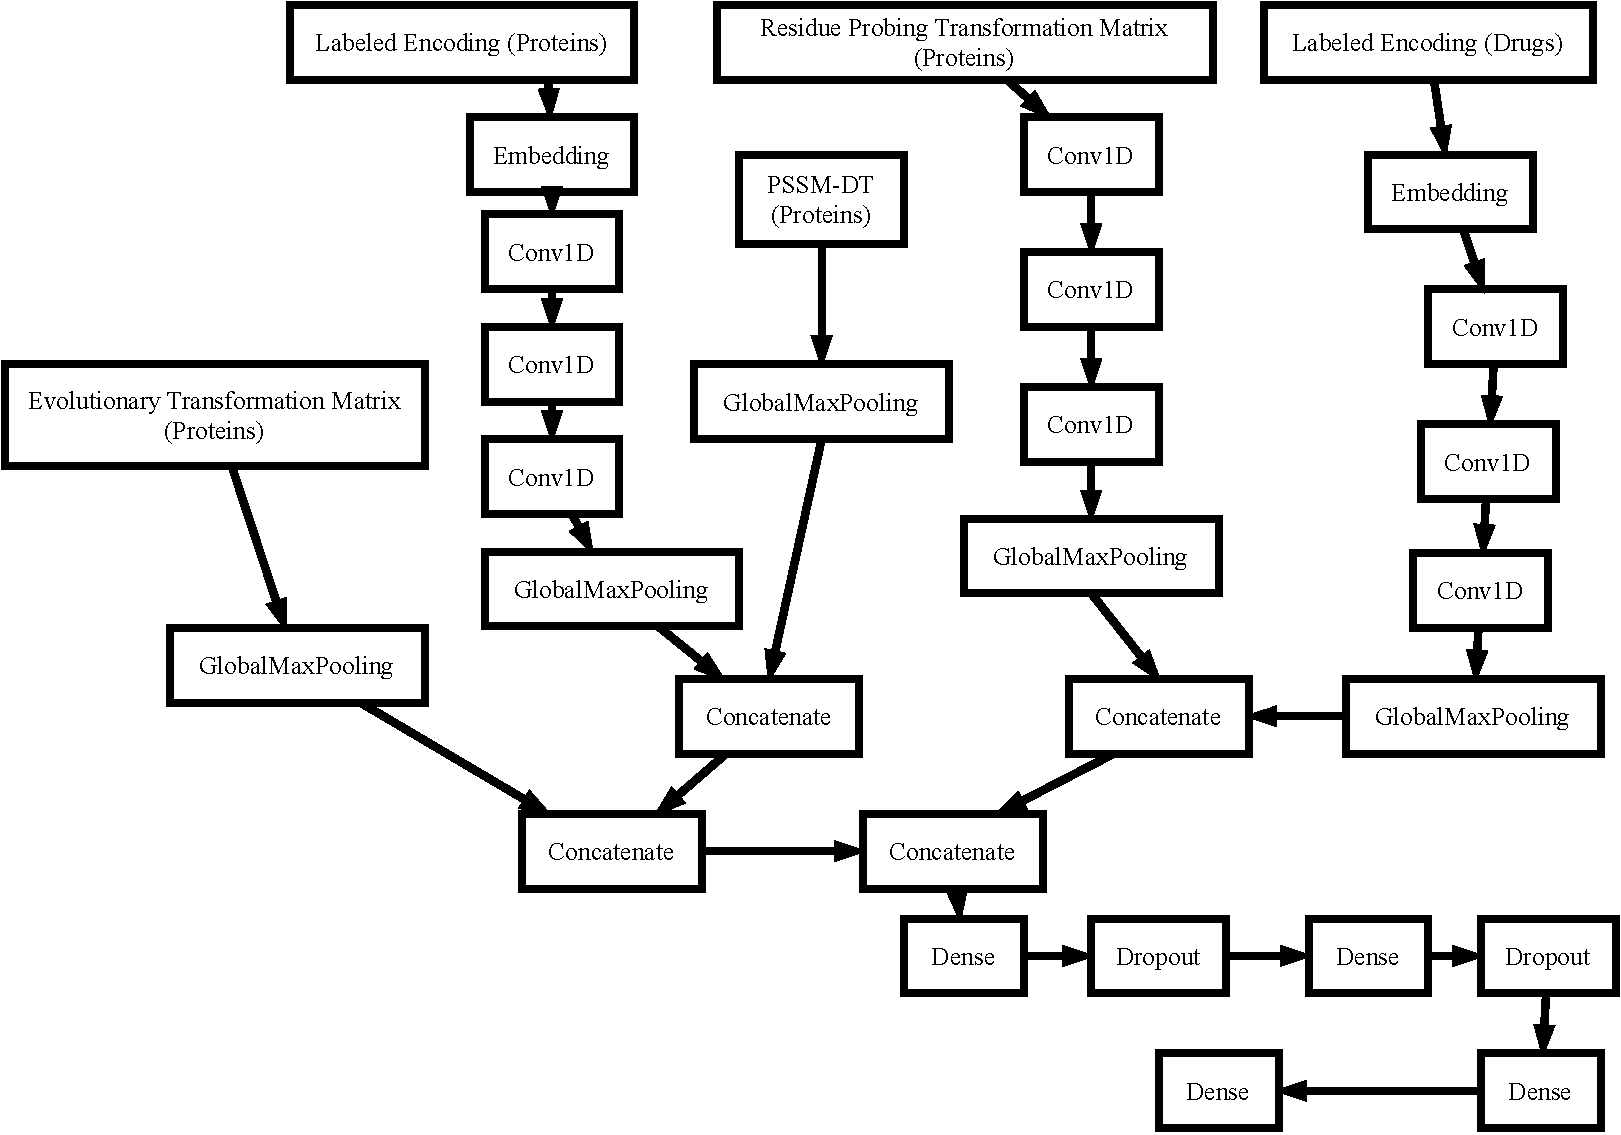
\includegraphics[width=1\linewidth]{mainmatter/3-Methodology/images/DeepDF_monchrome.pdf}
  \caption{Deep Learning Model to predict Protein-Drug Interaction}
  \label{fig:dlm}
  \end{figure}
  \begin{table}[H]\centering
    \caption{Inputs Used in the Deep Learning Network} 
    \begin{tabular}{|l|l|l|l|}
      \hline 
      S.No. & Input Layer Name & Used Feature Vector & Type \\ \hline
      1 & input\_1 & Label Encodings & Drug \\ \hline
      2 & input\_2 & Label Encodings & Protein \\ \hline
      3 & input\_3 & Evolutionary Distance Transformation Vector& Protein \\ \hline
      4 & input\_4 & PSSM-DT Vector & Protein \\ \hline
      5 & input\_5 & Residue Probing Transformation Vector & Protein \\   \hline 
    \end{tabular} 
    \label{table:inputs}
  \end{table}
  
  \subsection{Components description used from Tensorflow (Keras)}
  \subsubsection{Embedding Layer}
  From figure~\ref{fig:dlm}, the Embedding feature provided by keras for vector representation of both drug fingerprint and protein sequence are utilized. The label encodings of the drugs and protein sequences are inputs to this layer. It turns positive integers (indexes) into dense vectors of fixed size. eg. [[4], [20]] -> [[0.25, 0.1], [0.6, -0.2]].
 
  \subsubsection{Convolution Neural Network}
  \acrfull{cnn} are used for feature generation in machine learning system. They improve a machine learning system in three perspectives: sparse interactions, parameter sharing and equivariant representations. While a conventional neural network is tight network for instance, a Dense Layer creates an interaction of every input unit to that of output units; \acrshort{cnn} have sparse interactions. This differentiates the learning pattern of \acrshort{cnn} from other networks by understanding the local patterns in the input vector. While traditional Neural Networks mostly involve learning the global parameters, \acrshort{cnn} is used to learn local patterns. It does so by reducing the kernel (aka filter) smaller than the input. For example, when an image can have thousands of pixels, the kernel size can be tens or hundreds of pixels as shown in Figure ~\ref{fig:cnn}. 
  
  
  \begin{figure}[H]
    \centering
    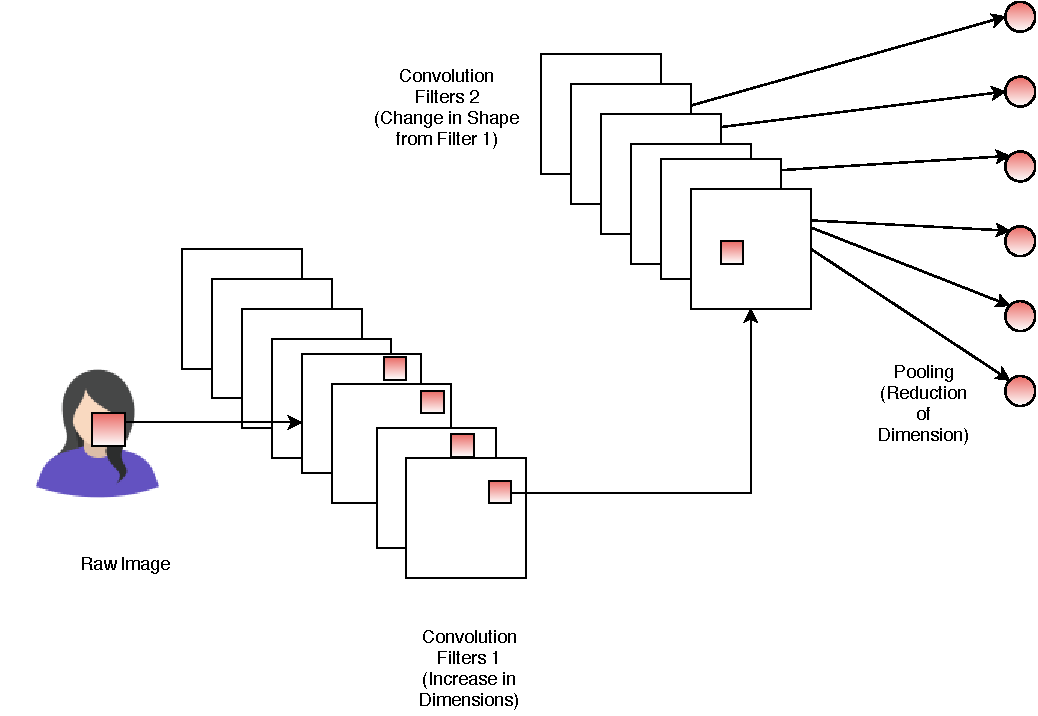
\includegraphics[width=1\linewidth]{mainmatter/3-Methodology/images/System-Block-CNN-Layer.pdf}
    \caption[Working of CNN Block]{Working of CNN Block:The small window from the image grid forms a filter. In first layer there is use of 8 filters}
    \label{fig:cnn}
  \end{figure}
  
  Parameter Sharing refers when the same parameter is used for multiple times in model. In conventional neural net, each parameter is used only once when computing the output of a layer. In \acrshort{cnn}, as the window sweeps over all the images, the same pixels create different representations with the position of sweeping window. So the parameter sharing property of \acrshort{cnn} identifies one representation for the pixel at a time.
  
  Equivariance property of \acrshort{cnn} is caused due to parameter sharing. It is defined as a property defined as when the input is translated, so is the output. When processing some time-series data the convolution produces a timeline sequence of features that appear in the input. For example, the convolution operations in movie will produce the feature timeline for the picture pixels.

  This research uses \acrfull{cnn} to learn the sequential representation of drug and proteins. As the primary structure of proteins and drugs are in fact representations of their 2D representations, the convolution operation will help to learn such features for further analysis. Again, 3D representations are also learned by higher layers of convolution layers. \citep{Adhikari2017}


\iffalse
  \begin{figure}[H]
    \centering
    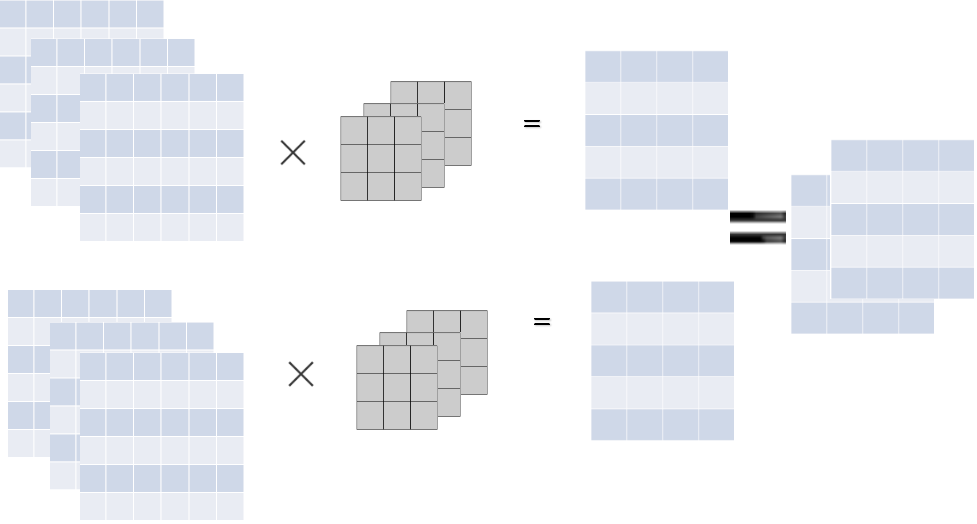
\includegraphics[width=.8\linewidth]{mainmatter/3-Methodology/images/cnn.png}
    \caption{Convolutional Neural Network}
    \label{fig:cnn}
  \end{figure} 
\fi


  
  
  \subsubsection{Pooling Layer}

  \begin{figure}[H] \centering
    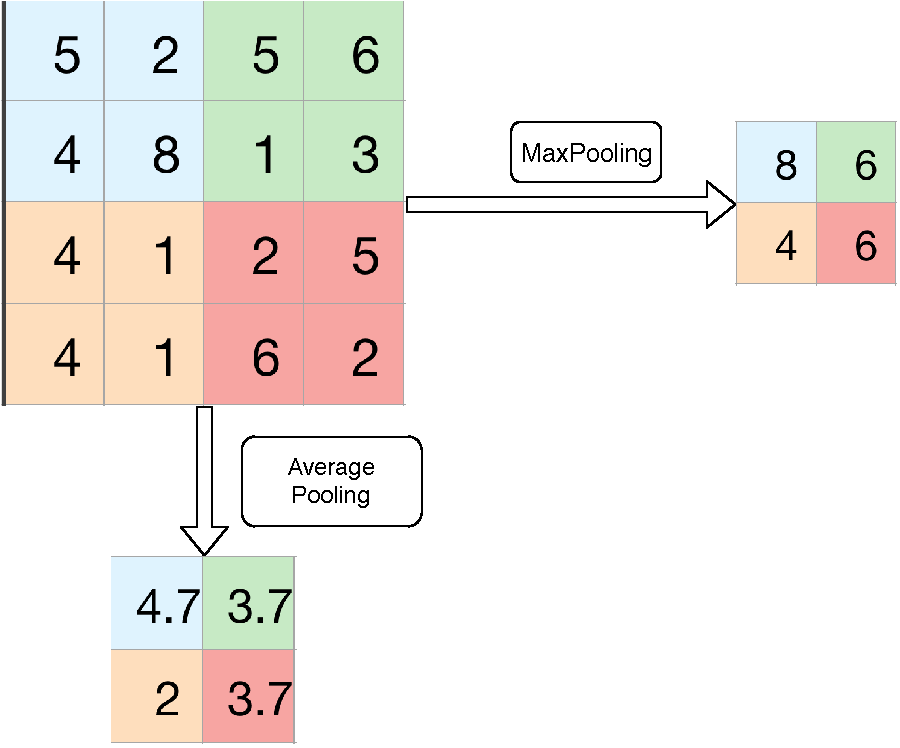
\includegraphics[width=.5\linewidth]{mainmatter/3-Methodology/images/pooling.pdf}
    \caption[Pooling Layer]{Pooling Layer: MaxPooling takes the maximum value from the pooling window and AveragePooling takes the mean from the pooling window.}
    \label{fig:pool_layer}
  \end{figure}

  
  The Pooling layer was used to modify the output of its preceding layer. For example the max pooling renders the maximum output from a rectangular neighborhood and average pooling renders average value from the the rectangular neighborhood. It was used to downsample the learned parameters from the grid of 2 dimensions returned by Convolution Layer. This work used Global Max Pooling to reduce the dimension and extract the extreme features learned from \acrshort{cnn}. Thus, it got reduced to 1 dimension by taking the highest values from the window size(corresponding to shape of 1\textsuperscript{st} dimensional element). The Pooling operation has been described by Figure ~\ref{fig:pool_layer}.

  
  \subsubsection{Dense Layer}
  Dense Layer is a neural layer which fully connects the input layer to output layer. It performs a linear operation on the layer's input vector. At every node in output of the dense layer generally follows an activation function that creates a generalization rule for the input vectors at the node. The research work used the dense layer to learn the global pattern from the feature data. The representation can be seen from Figure ~\ref{fig:dense}. As the output required is a regression value, it uses relu for activation.

  \begin{figure}[ht]
    \centering
    % 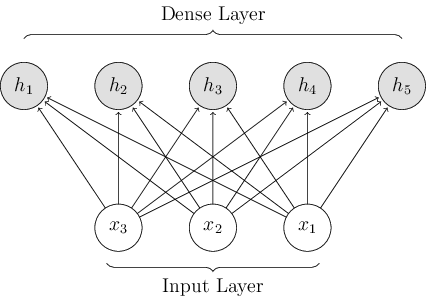
\includegraphics[width=.5\linewidth]{mainmatter/3-Methodology/images/dense.png}
    
  

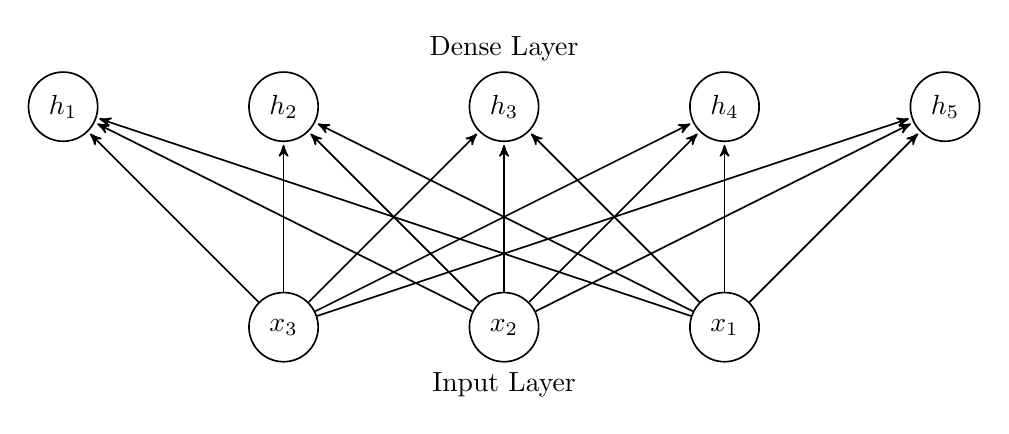
\begin{tikzpicture}[->,>=stealth',shorten >=1pt,auto,node distance=2.8cm,
    semithick]

      \tikzstyle{every state}=[text=black]
      \node[state]          (A)   {$h_1$};
      \node[state]         (B)  [right of=A] {$h_2$};
      \node[label=above:{Dense Layer},state]         (C) [right of=B] {$h_3$} ;
      \node[state]         (D) [right of=C] {$h_4$};
      \node[state]         (E) [right of=D] {$h_5$};

      \node[state]         (X1) [below of=B] {$x_3$};
      \node[state, label=below:{Input Layer}]         (X2) [right of=X1]       {$x_2$};
      \node[state]         (X3) [right of=X2]       {$x_1$};

      \path (X1) 
      edge              node {} (A)
      edge              node {} (B)
      edge              node {} (C)
      edge              node {} (D)
      edge              node {} (E)
      % edge              node {1,1,R} (C)
      (X2) 
      edge              node {} (A)
      edge              node {} (B)
      edge              node {} (C)
      edge              node {} (D)
      edge              node {} (E)
      % edge              node {0,1,L} (C)
      (X3)
      edge              node {} (A)
      edge              node {} (B)
      edge              node {} (C)
      edge              node {} (D)
      edge              node {} (E);
      % edge [bend left]  node {1,0,R} (E);

\end{tikzpicture}

  
\caption{Dense Layer}
\label{fig:dense}
\end{figure}

  
  \subsubsection{Dropout Layer}
  Our model becomes undesirable when every component of the input layer makes a significant change to the output layer. To reduce the effect of unimportant features the dropout layer was used. Thus the backpropagation network tries to ignore the noise features and minimizes the unrealizable prediction of the learning problem. This has been expressed diagrammatically in Figure ~\ref{fig:dropout}.
  \begin{figure}[tbh] \centering
    \captionsetup{justification=justified}
    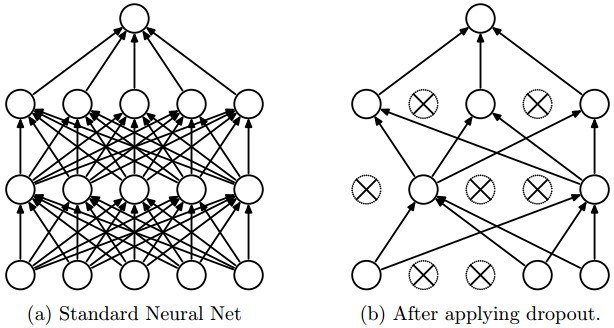
\includegraphics[width=.5\linewidth]{mainmatter/3-Methodology/images/dropout.jpeg}
    \caption[Dropout Layer]{a) Standard neural network whose all the nodes have weights connected to higher nodes and lower nodes. 
    b) Certain nodes belonging to same levels are disconnected. Some weights are also disconnected from other nodes depending on the percentage of dropout applied.}
    \label{fig:dropout}
  
  \end{figure}
  
  
  
  \subsubsection{Concatenation Layer}
  Concatenation Layer as the name implies is used to simply join two vectors so that a feature set comprising of multiple features can be created. Their positional index indicates the feature set being manipulated. The first dimensional length of input matrices and their no. of dimension should be same to concatenate the matrices.

  \subsubsection{Activation Layer}
  
  Activation Layer is a function that takes an input and provides an output based on the value. There are various kinds of Activation functions like Sigmoid, ReLu, Leaky Relu, tanh, Gaussian, Sinusoid etc. The research uses ReLu function for the activation layers.
  
  \subsubsection{Rectified Linear Unit}
  The output of Rectified Linear Unit (ReLu) is from 0 to infinity. For a normalized ReLu, the output will be between 0 to 1. The parametric equation is shown in Eq~\ref{eq:relu}.

  
  \begin{equation}
    f(x) = 
      \begin{cases}
        0 & ,for \quad x <= 0 \\
        x & ,for \quad x > 0
      \end{cases}
      \label{eq:relu}
  \end{equation}

  \begin{figure}
    \centering
    % \subfloat[ Relu Activation ][Relu Activation Function ]{
      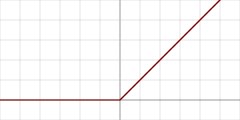
\includegraphics[width=.45\textwidth]{mainmatter/3-Methodology/images/relu.png}
    % }
    \label{fig:relu}
    \caption{Relu Activation Function}
  \end{figure}

   
  \subsection{Choice of Optimizers}

  Optimizers are the functions that estimate the global maximum/minimum for a problem domain. Their characteristics to find the global extremes or local extremes depend on the type of problem type and the optimization parameters used to train the algorithm. The choice of optimizer influences both the speed of convergence and whether it occurs. 
  The optimizers aim to minimize the cost function $ J( \theta; x^{(i)}; y^{(i)}) $ where $\theta$ is the optimization rule for cost function and $x{(i)},y{(i)}$ are the input,output parameters. The optimizers chosen to minimize the cost function associated to protein-drug prediction are:
  
  \subsubsection{Stochastic Gradient Descent(SGD)}

  The optimization formula for \acrfull{sgd}:
  \begin{equation}
    \theta = \theta - \eta \cdot \nabla_\theta J( \theta; x^{(i)}; y^{(i)})
  \end{equation}

  \subsubsection{Adaptive Moment Estimation(Adam)}

  The optimization formula for \acrfull{adam}:
  \begin{equation}
  \begin{aligned} V _ { d \theta } & = \beta _ { 1 } V _ { d \theta } + \left( 1 - \beta _ { 1 } \right) d \theta \\ S _ { d \theta } & = \beta _ { 2 } S _ { d \theta } + \left( 1 - \beta _ { 2 } \right) d \theta \\ V \operatorname { corr } _ { d \theta } & = \frac { V _ { d \theta } } { \left( 1 - \beta _ { 1 } \right) ^ { t } } \\ S c o r r _ { d \theta } & = \frac { S _ { d \theta } } { \left( 1 - \beta _ { 2 } \right) ^ { t } } \\ \theta & = \theta - \alpha \frac { d \theta } { \sqrt { S _ { d \theta } } + \varepsilon } \end{aligned}
  \end{equation}

  \subsubsection{Root Mean Squared Propagation(RMSProp)}

  \begin{equation}
    W_{dW} = \beta{W_{dW}} + (1-\beta) {\nabla\theta}^{2}
  \end{equation}

  \begin{equation}
    \theta = \theta - \eta \cdot \frac{\nabla_\theta}{\sqrt{W_{dW}} + \epsilon}  J( \theta; x^{(i)}; y^{(i)})
  \end{equation}


  \subsubsection{Adaptive Gradient Algorithm(AdaGrad)}
  
  \begin{equation}
    W_{dW} = \beta{W_{dW}} + (1-\beta) {\nabla\theta}
  \end{equation}

  \begin{equation}
    \theta = \theta - \eta \cdot W_{dW} J( \theta; x^{(i)}; y^{(i)})
  \end{equation}


  
  \iffalse
  \subsubsection{LSTM}
  As the \acrfull{rnn} often suffers from vanishing gradient problem~\footnote{Vanishing Gradient:During the training of RNN, the model vectors form a part of a loop and makes an unstable network.}, we use a \acrshort{lstm} Layer to learn the global pattern of the feature sets resulting after concatenation of different stacked layers outputs. The LSTM architecture can be seen in Figure ~\ref{fig:lstm}:
  \begin{figure} 
    [t]
    \centering
    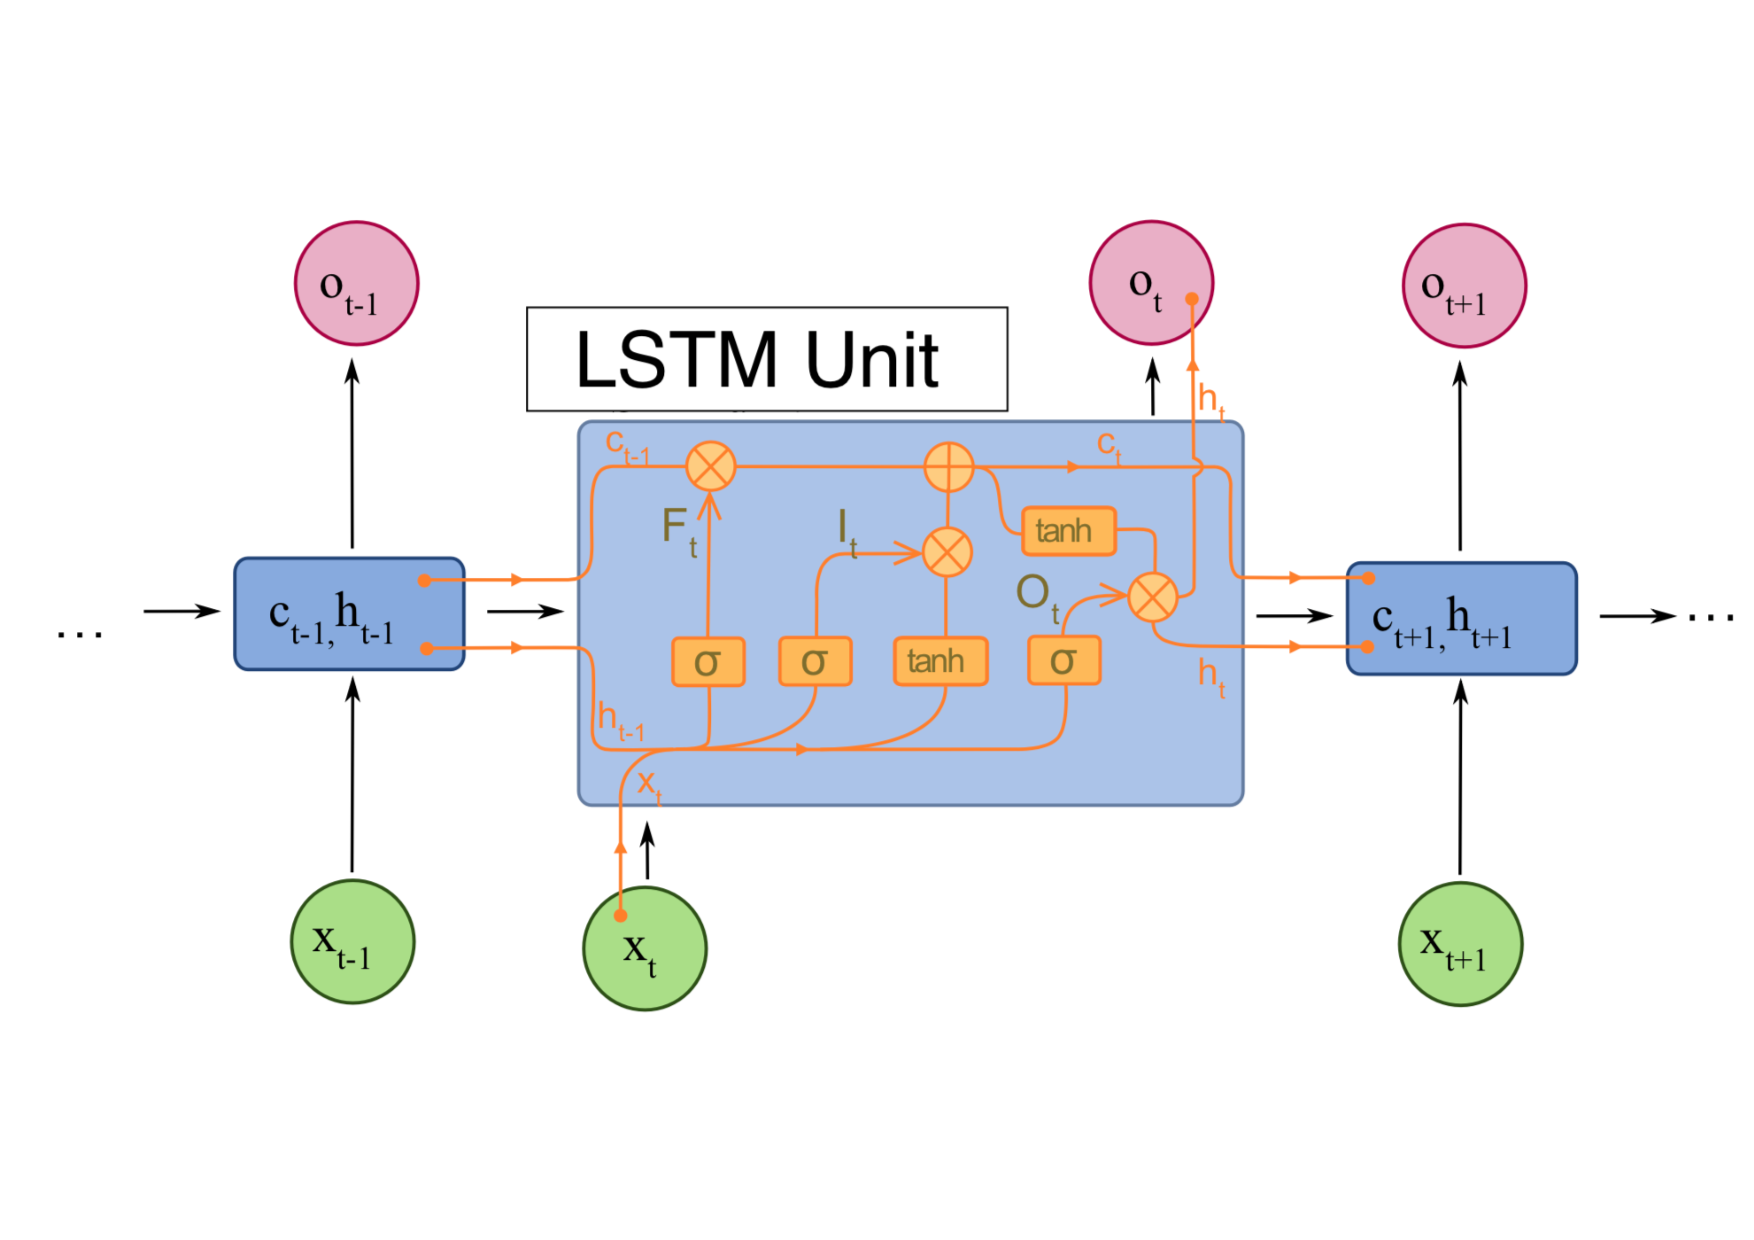
\includegraphics[width=1\linewidth]{mainmatter/3-Methodology/images/LSTM.pdf}
    \caption{Long Short Term Memory}
    \label{fig:lstm}
  \end{figure}
  In Figure~\ref{fig:lstm}, we can see that it contains a forget node, memory node and output node. These three nodes balance the information that needs to be removed, stored for future updates and necessarily fire the output node to make correct prediction.
  \fi